%%% The main file. It contains definitions of basic parameters and includes all other parts.

%% Settings for single-side (simplex) printing
% Margins: left 40mm, right 25mm, top and bottom 25mm
% (but beware, LaTeX adds 1in implicitly)
\documentclass[12pt,a4paper]{report}
\setlength\textwidth{145mm}
\setlength\textheight{247mm}
\setlength\oddsidemargin{15mm}
\setlength\evensidemargin{15mm}
\setlength\topmargin{0mm}
\setlength\headsep{0mm}
\setlength\headheight{0mm}
% \openright makes the following text appear on a right-hand page
\let\openright=\clearpage

%% Settings for two-sided (duplex) printing
% \documentclass[12pt,a4paper,twoside,openright]{report}
% \setlength\textwidth{145mm}
% \setlength\textheight{247mm}
% \setlength\oddsidemargin{14.2mm}
% \setlength\evensidemargin{0mm}
% \setlength\topmargin{0mm}
% \setlength\headsep{0mm}
% \setlength\headheight{0mm}
% \let\openright=\cleardoublepage

%% Generate PDF/A-2u
% \usepackage[a-2u]{pdfx}

%% Character encoding: usually latin2, cp1250 or utf8:
\usepackage[utf8]{inputenc}

%% Prefer Latin Modern fonts
\usepackage{lmodern}

\usepackage{makeidx}
\makeindex

%% Further useful packages (included in most LaTeX distributions)
\usepackage{amsmath}        % extensions for typesetting of math
% TODO: pick a font
\usepackage[charter]{mathdesign}
%\usepackage{millennial}
\usepackage[makeroom]{cancel}

\usepackage[usenames]{xcolor}  % typesetting in color
% \usepackage{amsfonts}       % math fonts
\usepackage{amsthm}         % theorems, definitions, etc.
\usepackage{bbding}         % various symbols (squares, asterisks, scissors, ...)
\usepackage{bm}             % boldface symbols (\bm)
\usepackage{graphicx}       % embedding of pictures
\usepackage{fancyvrb}       % improved verbatim environment
\usepackage{natbib}         % citation style AUTHOR (YEAR), or AUTHOR [NUMBER]
\usepackage[nottoc]{tocbibind} % makes sure that bibliography and the lists
                               % of figures/tables are included in the table
                               % of contents
\usepackage{dcolumn}        % improved alignment of table columns
\usepackage{booktabs}       % improved horizontal lines in tables
\usepackage{paralist}       % improved enumerate and itemize
\usepackage[colorinlistoftodos,prependcaption,textsize=tiny]{todonotes}
\usepackage{tcolorbox}

\usepackage{hyperref}
\usepackage{url}


% \usepackage{mathtools}
% \DeclarePairedDelimiterX{\infdivx}[2]{(}{)}{%
%   #1\;\delimsize\|\;#2%
% }
% \DeclarePairedDelimiter{\norm}{\lVert}{\rVert}

\newcommand{\kldiv}{D_{KL}\infdivx}

\usepackage{braket}

\newlength{\notationgap}
\setlength{\notationgap}{1pc}

%%%%% NEW MATH DEFINITIONS %%%%%

% Mark sections of captions for referring to divisions of figures
\newcommand{\figleft}{{\em (Left)}}
\newcommand{\figcenter}{{\em (Center)}}
\newcommand{\figright}{{\em (Right)}}
\newcommand{\figtop}{{\em (Top)}}
\newcommand{\figbottom}{{\em (Bottom)}}
\newcommand{\captiona}{{\em (a)}}
\newcommand{\captionb}{{\em (b)}}
\newcommand{\captionc}{{\em (c)}}
\newcommand{\captiond}{{\em (d)}}

% Highlight a newly defined term
\newcommand{\newterm}[1]{{\bf #1 \index{#1}}}


% Figure reference, lower-case.
\def\figref#1{figure~\ref{#1}}
% Figure reference, capital. For start of sentence
\def\Figref#1{Figure~\ref{#1}}
\def\twofigref#1#2{figures \ref{#1} and \ref{#2}}
\def\quadfigref#1#2#3#4{figures \ref{#1}, \ref{#2}, \ref{#3} and \ref{#4}}
% Section reference, lower-case.
\def\secref#1{section~\ref{#1}}
% Section reference, capital.
\def\Secref#1{Section~\ref{#1}}
% Reference to two sections.
\def\twosecrefs#1#2{sections \ref{#1} and \ref{#2}}
% Reference to three sections.
\def\secrefs#1#2#3{sections \ref{#1}, \ref{#2} and \ref{#3}}
% Reference to an equation, lower-case.
\def\eqref#1{equation~\ref{#1}}
% Reference to an equation, upper case
\def\Eqref#1{Equation~\ref{#1}}
% A raw reference to an equation---avoid using if possible
\def\plaineqref#1{\ref{#1}}
% Reference to a chapter, lower-case.
\def\chapref#1{chapter~\ref{#1}}
% Reference to an equation, upper case.
\def\Chapref#1{Chapter~\ref{#1}}
% Reference to a range of chapters
\def\rangechapref#1#2{chapters\ref{#1}--\ref{#2}}
% Reference to an algorithm, lower-case.
\def\algref#1{algorithm~\ref{#1}}
% Reference to an algorithm, upper case.
\def\Algref#1{Algorithm~\ref{#1}}
\def\twoalgref#1#2{algorithms \ref{#1} and \ref{#2}}
\def\Twoalgref#1#2{Algorithms \ref{#1} and \ref{#2}}
% Reference to a part, lower case
\def\partref#1{part~\ref{#1}}
% Reference to a part, upper case
\def\Partref#1{Part~\ref{#1}}
\def\twopartref#1#2{parts \ref{#1} and \ref{#2}}

\def\ceil#1{\lceil #1 \rceil}
\def\floor#1{\lfloor #1 \rfloor}
\def\1{\bm{1}}
\newcommand{\train}{\mathcal{D}}
\newcommand{\valid}{\mathcal{D_{\mathrm{valid}}}}
\newcommand{\test}{\mathcal{D_{\mathrm{test}}}}

\def\eps{{\epsilon}}

% Covariance matrix helpers
\def\ms#1{{\mSigma_{#1}}}
\def\ml#1{{\mLambda_{#1}}}

% Partition matrix helpers

\def\partx{{\begin{bmatrix} \vx_1 \\ \vx_2 \end{bmatrix}}}
\def\partmu{{\begin{bmatrix} \vmu_1 \\ \vmu_2 \end{bmatrix}}}
\def\partxmu{{\begin{bmatrix} \vx_1 - \vmu_1 \\ \vx_2 - \vmu_2 \end{bmatrix}}}
\def\partsigma{{\begin{bmatrix} \ms{11} & \ms{12} \\ \ms{21} & \ms{22} \end{bmatrix}}}
\def\partlambda{{\begin{bmatrix} \ml{11} & \ml{12} \\ \ml{21} & \ml{22} \end{bmatrix}}}

% Random variables
\def\reta{{\textnormal{$\eta$}}}
\def\ra{{\textnormal{a}}}
\def\rb{{\textnormal{b}}}
\def\rc{{\textnormal{c}}}
\def\rd{{\textnormal{d}}}
\def\re{{\textnormal{e}}}
\def\rf{{\textnormal{f}}}
\def\rg{{\textnormal{g}}}
\def\rh{{\textnormal{h}}}
\def\ri{{\textnormal{i}}}
\def\rj{{\textnormal{j}}}
\def\rk{{\textnormal{k}}}
\def\rl{{\textnormal{l}}}
% rm is already a command, just don't name any random variables m
\def\rn{{\textnormal{n}}}
\def\ro{{\textnormal{o}}}
\def\rp{{\textnormal{p}}}
\def\rq{{\textnormal{q}}}
\def\rr{{\textnormal{r}}}
\def\rs{{\textnormal{s}}}
\def\rt{{\textnormal{t}}}
\def\ru{{\textnormal{u}}}
\def\rv{{\textnormal{v}}}
\def\rw{{\textnormal{w}}}
\def\rx{{\textnormal{x}}}
\def\ry{{\textnormal{y}}}
\def\rz{{\textnormal{z}}}

% Random vectors
\def\rvepsilon{{\mathbf{\epsilon}}}
\def\rvtheta{{\mathbf{\theta}}}
\def\rva{{\mathbf{a}}}
\def\rvb{{\mathbf{b}}}
\def\rvc{{\mathbf{c}}}
\def\rvd{{\mathbf{d}}}
\def\rve{{\mathbf{e}}}
\def\rvf{{\mathbf{f}}}
\def\rvg{{\mathbf{g}}}
\def\rvh{{\mathbf{h}}}
\def\rvu{{\mathbf{i}}}
\def\rvj{{\mathbf{j}}}
\def\rvk{{\mathbf{k}}}
\def\rvl{{\mathbf{l}}}
\def\rvm{{\mathbf{m}}}
\def\rvn{{\mathbf{n}}}
\def\rvo{{\mathbf{o}}}
\def\rvp{{\mathbf{p}}}
\def\rvq{{\mathbf{q}}}
\def\rvr{{\mathbf{r}}}
\def\rvs{{\mathbf{s}}}
\def\rvt{{\mathbf{t}}}
\def\rvu{{\mathbf{u}}}
\def\rvv{{\mathbf{v}}}
\def\rvw{{\mathbf{w}}}
\def\rvx{{\mathbf{x}}}
\def\rvy{{\mathbf{y}}}
\def\rvz{{\mathbf{z}}}

% Elements of random vectors
\def\erva{{\textnormal{a}}}
\def\ervb{{\textnormal{b}}}
\def\ervc{{\textnormal{c}}}
\def\ervd{{\textnormal{d}}}
\def\erve{{\textnormal{e}}}
\def\ervf{{\textnormal{f}}}
\def\ervg{{\textnormal{g}}}
\def\ervh{{\textnormal{h}}}
\def\ervi{{\textnormal{i}}}
\def\ervj{{\textnormal{j}}}
\def\ervk{{\textnormal{k}}}
\def\ervl{{\textnormal{l}}}
\def\ervm{{\textnormal{m}}}
\def\ervn{{\textnormal{n}}}
\def\ervo{{\textnormal{o}}}
\def\ervp{{\textnormal{p}}}
\def\ervq{{\textnormal{q}}}
\def\ervr{{\textnormal{r}}}
\def\ervs{{\textnormal{s}}}
\def\ervt{{\textnormal{t}}}
\def\ervu{{\textnormal{u}}}
\def\ervv{{\textnormal{v}}}
\def\ervw{{\textnormal{w}}}
\def\ervx{{\textnormal{x}}}
\def\ervy{{\textnormal{y}}}
\def\ervz{{\textnormal{z}}}

% Random matrices
\def\rmA{{\mathbf{A}}}
\def\rmB{{\mathbf{B}}}
\def\rmC{{\mathbf{C}}}
\def\rmD{{\mathbf{D}}}
\def\rmE{{\mathbf{E}}}
\def\rmF{{\mathbf{F}}}
\def\rmG{{\mathbf{G}}}
\def\rmH{{\mathbf{H}}}
\def\rmI{{\mathbf{I}}}
\def\rmJ{{\mathbf{J}}}
\def\rmK{{\mathbf{K}}}
\def\rmL{{\mathbf{L}}}
\def\rmM{{\mathbf{M}}}
\def\rmN{{\mathbf{N}}}
\def\rmO{{\mathbf{O}}}
\def\rmP{{\mathbf{P}}}
\def\rmQ{{\mathbf{Q}}}
\def\rmR{{\mathbf{R}}}
\def\rmS{{\mathbf{S}}}
\def\rmT{{\mathbf{T}}}
\def\rmU{{\mathbf{U}}}
\def\rmV{{\mathbf{V}}}
\def\rmW{{\mathbf{W}}}
\def\rmX{{\mathbf{X}}}
\def\rmY{{\mathbf{Y}}}
\def\rmZ{{\mathbf{Z}}}

% Elements of random matrices
\def\ermA{{\textnormal{A}}}
\def\ermB{{\textnormal{B}}}
\def\ermC{{\textnormal{C}}}
\def\ermD{{\textnormal{D}}}
\def\ermE{{\textnormal{E}}}
\def\ermF{{\textnormal{F}}}
\def\ermG{{\textnormal{G}}}
\def\ermH{{\textnormal{H}}}
\def\ermI{{\textnormal{I}}}
\def\ermJ{{\textnormal{J}}}
\def\ermK{{\textnormal{K}}}
\def\ermL{{\textnormal{L}}}
\def\ermM{{\textnormal{M}}}
\def\ermN{{\textnormal{N}}}
\def\ermO{{\textnormal{O}}}
\def\ermP{{\textnormal{P}}}
\def\ermQ{{\textnormal{Q}}}
\def\ermR{{\textnormal{R}}}
\def\ermS{{\textnormal{S}}}
\def\ermT{{\textnormal{T}}}
\def\ermU{{\textnormal{U}}}
\def\ermV{{\textnormal{V}}}
\def\ermW{{\textnormal{W}}}
\def\ermX{{\textnormal{X}}}
\def\ermY{{\textnormal{Y}}}
\def\ermZ{{\textnormal{Z}}}

% Vectors
\def\vzero{{\bm{0}}}
\def\vone{{\bm{1}}}
\def\vmu{{\bm{\mu}}}
\def\vtheta{{\bm{\theta}}}
\def\va{{\bm{a}}}
\def\vb{{\bm{b}}}
\def\vc{{\bm{c}}}
\def\vd{{\bm{d}}}
\def\ve{{\bm{e}}}
\def\vf{{\bm{f}}}
\def\vg{{\bm{g}}}
\def\vh{{\bm{h}}}
\def\vi{{\bm{i}}}
\def\vj{{\bm{j}}}
\def\vk{{\bm{k}}}
\def\vl{{\bm{l}}}
\def\vm{{\bm{m}}}
\def\vn{{\bm{n}}}
\def\vo{{\bm{o}}}
\def\vp{{\bm{p}}}
\def\vq{{\bm{q}}}
\def\vr{{\bm{r}}}
\def\vs{{\bm{s}}}
\def\vt{{\bm{t}}}
\def\vu{{\bm{u}}}
\def\vv{{\bm{v}}}
\def\vw{{\bm{w}}}
\def\vx{{\bm{x}}}
\def\vy{{\bm{y}}}
\def\vz{{\bm{z}}}

% Elements of vectors
\def\evalpha{{\alpha}}
\def\evbeta{{\beta}}
\def\evepsilon{{\epsilon}}
\def\evlambda{{\lambda}}
\def\evomega{{\omega}}
\def\evmu{{\mu}}
\def\evpsi{{\psi}}
\def\evsigma{{\sigma}}
\def\evtheta{{\theta}}
\def\eva{{a}}
\def\evb{{b}}
\def\evc{{c}}
\def\evd{{d}}
\def\eve{{e}}
\def\evf{{f}}
\def\evg{{g}}
\def\evh{{h}}
\def\evi{{i}}
\def\evj{{j}}
\def\evk{{k}}
\def\evl{{l}}
\def\evm{{m}}
\def\evn{{n}}
\def\evo{{o}}
\def\evp{{p}}
\def\evq{{q}}
\def\evr{{r}}
\def\evs{{s}}
\def\evt{{t}}
\def\evu{{u}}
\def\evv{{v}}
\def\evw{{w}}
\def\evx{{x}}
\def\evy{{y}}
\def\evz{{z}}

% Matrix
\def\mA{{\bm{A}}}
\def\mB{{\bm{B}}}
\def\mC{{\bm{C}}}
\def\mD{{\bm{D}}}
\def\mE{{\bm{E}}}
\def\mF{{\bm{F}}}
\def\mG{{\bm{G}}}
\def\mH{{\bm{H}}}
\def\mI{{\bm{I}}}
\def\mJ{{\bm{J}}}
\def\mK{{\bm{K}}}
\def\mL{{\bm{L}}}
\def\mM{{\bm{M}}}
\def\mN{{\bm{N}}}
\def\mO{{\bm{O}}}
\def\mP{{\bm{P}}}
\def\mQ{{\bm{Q}}}
\def\mR{{\bm{R}}}
\def\mS{{\bm{S}}}
\def\mT{{\bm{T}}}
\def\mU{{\bm{U}}}
\def\mV{{\bm{V}}}
\def\mW{{\bm{W}}}
\def\mX{{\bm{X}}}
\def\mY{{\bm{Y}}}
\def\mZ{{\bm{Z}}}
\def\mBeta{{\bm{\beta}}}
\def\mPhi{{\bm{\Phi}}}
\def\mLambda{{\bm{\Lambda}}}
\def\mSigma{{\bm{\Sigma}}}
\def\mZero{{\bm{0}}}

% Tensor
\DeclareMathAlphabet{\mathsfit}{\encodingdefault}{\sfdefault}{m}{sl}
\SetMathAlphabet{\mathsfit}{bold}{\encodingdefault}{\sfdefault}{bx}{n}
\newcommand{\tens}[1]{\bm{\mathsfit{#1}}}
\def\tA{{\tens{A}}}
\def\tB{{\tens{B}}}
\def\tC{{\tens{C}}}
\def\tD{{\tens{D}}}
\def\tE{{\tens{E}}}
\def\tF{{\tens{F}}}
\def\tG{{\tens{G}}}
\def\tH{{\tens{H}}}
\def\tI{{\tens{I}}}
\def\tJ{{\tens{J}}}
\def\tK{{\tens{K}}}
\def\tL{{\tens{L}}}
\def\tM{{\tens{M}}}
\def\tN{{\tens{N}}}
\def\tO{{\tens{O}}}
\def\tP{{\tens{P}}}
\def\tQ{{\tens{Q}}}
\def\tR{{\tens{R}}}
\def\tS{{\tens{S}}}
\def\tT{{\tens{T}}}
\def\tU{{\tens{U}}}
\def\tV{{\tens{V}}}
\def\tW{{\tens{W}}}
\def\tX{{\tens{X}}}
\def\tY{{\tens{Y}}}
\def\tZ{{\tens{Z}}}


% Graph
\def\gA{{\mathcal{A}}}
\def\gB{{\mathcal{B}}}
\def\gC{{\mathcal{C}}}
\def\gD{{\mathcal{D}}}
\def\gE{{\mathcal{E}}}
\def\gF{{\mathcal{F}}}
\def\gG{{\mathcal{G}}}
\def\gH{{\mathcal{H}}}
\def\gI{{\mathcal{I}}}
\def\gJ{{\mathcal{J}}}
\def\gK{{\mathcal{K}}}
\def\gL{{\mathcal{L}}}
\def\gM{{\mathcal{M}}}
\def\gN{{\mathcal{N}}}
\def\gO{{\mathcal{O}}}
\def\gP{{\mathcal{P}}}
\def\gQ{{\mathcal{Q}}}
\def\gR{{\mathcal{R}}}
\def\gS{{\mathcal{S}}}
\def\gT{{\mathcal{T}}}
\def\gU{{\mathcal{U}}}
\def\gV{{\mathcal{V}}}
\def\gW{{\mathcal{W}}}
\def\gX{{\mathcal{X}}}
\def\gY{{\mathcal{Y}}}
\def\gZ{{\mathcal{Z}}}

% Sets
\def\sA{{\mathbb{A}}}
\def\sB{{\mathbb{B}}}
\def\sC{{\mathbb{C}}}
\def\sD{{\mathbb{D}}}
% Don't use a set called E, because this would be the same as our symbol
% for expectation.
\def\sF{{\mathbb{F}}}
\def\sG{{\mathbb{G}}}
\def\sH{{\mathbb{H}}}
\def\sI{{\mathbb{I}}}
\def\sJ{{\mathbb{J}}}
\def\sK{{\mathbb{K}}}
\def\sL{{\mathbb{L}}}
\def\sM{{\mathbb{M}}}
\def\sN{{\mathbb{N}}}
\def\sO{{\mathbb{O}}}
\def\sP{{\mathbb{P}}}
\def\sQ{{\mathbb{Q}}}
\def\sR{{\mathbb{R}}}
\def\sS{{\mathbb{S}}}
\def\sT{{\mathbb{T}}}
\def\sU{{\mathbb{U}}}
\def\sV{{\mathbb{V}}}
\def\sW{{\mathbb{W}}}
\def\sX{{\mathbb{X}}}
\def\sY{{\mathbb{Y}}}
\def\sZ{{\mathbb{Z}}}

% Entries of a matrix
\def\emLambda{{\Lambda}}
\def\emA{{A}}
\def\emB{{B}}
\def\emC{{C}}
\def\emD{{D}}
\def\emE{{E}}
\def\emF{{F}}
\def\emG{{G}}
\def\emH{{H}}
\def\emI{{I}}
\def\emJ{{J}}
\def\emK{{K}}
\def\emL{{L}}
\def\emM{{M}}
\def\emN{{N}}
\def\emO{{O}}
\def\emP{{P}}
\def\emQ{{Q}}
\def\emR{{R}}
\def\emS{{S}}
\def\emT{{T}}
\def\emU{{U}}
\def\emV{{V}}
\def\emW{{W}}
\def\emX{{X}}
\def\emY{{Y}}
\def\emZ{{Z}}
\def\emSigma{{\Sigma}}

% entries of a tensor
% Same font as tensor, without \bm wrapper
\newcommand{\etens}[1]{\mathsfit{#1}}
\def\etLambda{{\etens{\Lambda}}}
\def\etA{{\etens{A}}}
\def\etB{{\etens{B}}}
\def\etC{{\etens{C}}}
\def\etD{{\etens{D}}}
\def\etE{{\etens{E}}}
\def\etF{{\etens{F}}}
\def\etG{{\etens{G}}}
\def\etH{{\etens{H}}}
\def\etI{{\etens{I}}}
\def\etJ{{\etens{J}}}
\def\etK{{\etens{K}}}
\def\etL{{\etens{L}}}
\def\etM{{\etens{M}}}
\def\etN{{\etens{N}}}
\def\etO{{\etens{O}}}
\def\etP{{\etens{P}}}
\def\etQ{{\etens{Q}}}
\def\etR{{\etens{R}}}
\def\etS{{\etens{S}}}
\def\etT{{\etens{T}}}
\def\etU{{\etens{U}}}
\def\etV{{\etens{V}}}
\def\etW{{\etens{W}}}
\def\etX{{\etens{X}}}
\def\etY{{\etens{Y}}}
\def\etZ{{\etens{Z}}}

% The true underlying data generating distribution
\newcommand{\pdata}{p_{\rm{data}}}
% The empirical distribution defined by the training set
\newcommand{\ptrain}{\hat{p}_{\rm{data}}}
\newcommand{\Ptrain}{\hat{P}_{\rm{data}}}
% The model distribution
\newcommand{\pmodel}{p_{\rm{model}}}
\newcommand{\Pmodel}{P_{\rm{model}}}
\newcommand{\ptildemodel}{\tilde{p}_{\rm{model}}}
% Stochastic autoencoder distributions
\newcommand{\pencode}{p_{\rm{encoder}}}
\newcommand{\pdecode}{p_{\rm{decoder}}}
\newcommand{\precons}{p_{\rm{reconstruct}}}

\newcommand{\laplace}{\mathrm{Laplace}} % Laplace distribution

\newcommand*\diff{\mathop{}\!\mathrm{d}}
\newcommand*\Diff[1]{\mathop{}\!\mathrm{d^#1}}
\newcommand{\dx}{\diff x}

% TODO: why is \E and \R already defined?
%\newcommand{\E}{\mathbb{E}}
\newcommand{\Ls}{\mathcal{L}}
%\newcommand{\R}{\mathbb{R}}
\newcommand{\emp}{\tilde{p}}
\newcommand{\lr}{\alpha}
\newcommand{\reg}{\lambda}
\newcommand{\rect}{\mathrm{rectifier}}
\newcommand{\softmax}{\mathrm{softmax}}
\newcommand{\sigmoid}{\sigma}
\newcommand{\softplus}{\zeta}
\newcommand{\KL}{D_{\mathrm{KL}}}
\newcommand{\Var}{\mathrm{Var}}
\newcommand{\standarderror}{\mathrm{SE}}
\newcommand{\Cov}{\mathrm{Cov}}
% Wolfram Mathworld says $L^2$ is for function spaces and $\ell^2$ is for vectors
% But then they seem to use $L^2$ for vectors throughout the site, and so does
% wikipedia.
\newcommand{\normlzero}{L^0}
\newcommand{\normlone}{L^1}
\newcommand{\normltwo}{L^2}
\newcommand{\normlp}{L^p}
\newcommand{\normmax}{L^\infty}

\newcommand{\parents}{Pa} % See usage in notation.tex. Chosen to match Daphne's book.

\DeclareMathOperator*{\argmax}{arg\,max}
\DeclareMathOperator*{\argmin}{arg\,min}

\DeclareMathOperator{\sign}{sign}
\DeclareMathOperator{\Tr}{Tr}
\let\ab\allowbreak


% \usepackage{unicode-math}

%%% Basic information on the thesis

% Thesis title in English (exactly as in the formal assignment)
\def\ThesisTitle{Thesis title}

% Author of the thesis
\def\ThesisAuthor{Jakub Arnold}

% Year when the thesis is submitted
\def\YearSubmitted{YEAR}

% Name of the department or institute, where the work was officially assigned
% (according to the Organizational Structure of MFF UK in English,
% or a full name of a department outside MFF)
\def\Department{Institute of Formal and Applied Linguistics}

% Is it a department (katedra), or an institute (ústav)?
\def\DeptType{Institute}

% Thesis supervisor: name, surname and titles
\def\Supervisor{RNDr. Milan Straka, Ph.D.}

% Supervisor's department (again according to Organizational structure of MFF)
\def\SupervisorsDepartment{Institute of Formal and Applied Linguistics}

% Study programme and specialization
\def\StudyProgramme{Computer Science}
\def\StudyBranch{Artificial Intelligence}

% An optional dedication: you can thank whomever you wish (your supervisor,
% consultant, a person who lent the software, etc.)
\def\Dedication{%
Dedication.
}

% Abstract (recommended length around 80-200 words; this is not a copy of your thesis assignment!)
\def\Abstract{%
Abstract.
}

% 3 to 5 keywords (recommended), each enclosed in curly braces
\def\Keywords{%
{key} {words}
}

%% The hyperref package for clickable links in PDF and also for storing
%% metadata to PDF (including the table of contents).
%% Most settings are pre-set by the pdfx package.
\hypersetup{unicode}
\hypersetup{breaklinks=true}

% Definitions of macros (see description inside)
%%% This file contains definitions of various useful macros and environments %%%
%%% Please add more macros here instead of cluttering other files with them. %%%

%%% Minor tweaks of style

% These macros employ a little dirty trick to convince LaTeX to typeset
% chapter headings sanely, without lots of empty space above them.
% Feel free to ignore.
\makeatletter
\def\@makechapterhead#1{
  {\parindent \z@ \raggedright \normalfont
   \Huge\bfseries \thechapter. #1
   \par\nobreak
   \vskip 20\p@
}}
\def\@makeschapterhead#1{
  {\parindent \z@ \raggedright \normalfont
   \Huge\bfseries #1
   \par\nobreak
   \vskip 20\p@
}}
\makeatother

% This macro defines a chapter, which is not numbered, but is included
% in the table of contents.
\def\chapwithtoc#1{
\chapter*{#1}
\addcontentsline{toc}{chapter}{#1}
}

% Draw black "slugs" whenever a line overflows, so that we can spot it easily.
\overfullrule=0mm

%%% Macros for definitions, theorems, claims, examples, ... (requires amsthm package)

\theoremstyle{plain}
\newtheorem{thm}{Theorem}
\newtheorem{lemma}[thm]{Lemma}
\newtheorem{claim}[thm]{Claim}

\theoremstyle{plain}
\newtheorem{defn}{Definition}

\theoremstyle{remark}
\newtheorem*{cor}{Corollary}
\newtheorem*{rem}{Remark}
\newtheorem*{example}{Example}

%%% An environment for proofs

%%% FIXME %%% \newenvironment{proof}{
%%% FIXME %%%   \par\medskip\noindent
%%% FIXME %%%   \textit{Proof}.
%%% FIXME %%% }{
%%% FIXME %%% \newline
%%% FIXME %%% \rightline{$\square$}  % or \SquareCastShadowBottomRight from bbding package
%%% FIXME %%% }

%%% An environment for typesetting of program code and input/output
%%% of programs. (Requires the fancyvrb package -- fancy verbatim.)

\DefineVerbatimEnvironment{code}{Verbatim}{fontsize=\small, frame=single}

%%% The field of all real and natural numbers
\newcommand{\R}{\mathbb{R}}
\newcommand{\N}{\mathbb{N}}

%%% Useful operators for statistics and probability
\DeclareMathOperator{\pr}{\textsf{P}}
\DeclareMathOperator{\E}{\textsf{E}\,}
\DeclareMathOperator{\var}{\textrm{var}}
\DeclareMathOperator{\sd}{\textrm{sd}}

%%% Transposition of a vector/matrix
\newcommand{\T}[1]{#1^\top}

%%% Various math goodies
\newcommand{\goto}{\rightarrow}
\newcommand{\gotop}{\stackrel{P}{\longrightarrow}}
\newcommand{\maon}[1]{o(n^{#1})}
\newcommand{\abs}[1]{\left|{#1}\right|}
\newcommand{\dint}{\int_0^\tau\!\!\int_0^\tau}
\newcommand{\isqr}[1]{\frac{1}{\sqrt{#1}}}

%%% Various table goodies
\newcommand{\pulrad}[1]{\raisebox{1.5ex}[0pt]{#1}}
\newcommand{\mc}[1]{\multicolumn{1}{c}{#1}}

%%% Uppercase autoref labels
\renewcommand{\footnoteautorefname}{Footnote}
\renewcommand{\itemautorefname}{Item}
\renewcommand{\chapterautorefname}{Chapter}
\renewcommand{\sectionautorefname}{Section}
\renewcommand{\subsectionautorefname}{Subsection}
\renewcommand{\subsubsectionautorefname}{Subsubsection}
\renewcommand{\paragraphautorefname}{Paragraph}
\renewcommand{\subparagraphautorefname}{Subparagraph}
\renewcommand{\FancyVerbLineautorefname}{Line}
\renewcommand{\pageautorefname}{Page}
\renewcommand{\algorithmautorefname}{Algorithm}


% Title page and various mandatory informational pages
\begin{document}
% TODO: tohle smazat?
\title{Master Thesis}

%%% Title page of the thesis and other mandatory pages

%%% Title page of the thesis

\pagestyle{empty}
\hypersetup{pageanchor=false}
\begin{center}

\centerline{\mbox{
\includegraphics[width=166mm]{img/logo-en.pdf}}}

\vspace{-8mm}
\vfill

{\bf\Large MASTER THESIS}

\vfill

{\LARGE\ThesisAuthor}

\vspace{15mm}

{\LARGE\bfseries\ThesisTitle}

\vfill

\Department

\vfill

\begin{tabular}{rl}

Supervisor of the master thesis: & \Supervisor \\
\noalign{\vspace{2mm}}
Study programme: & \StudyProgramme \\
\noalign{\vspace{2mm}}
Study branch: & \StudyBranch \\
\end{tabular}

\vfill

% Zde doplňte rok
Prague \YearSubmitted

\end{center}

\newpage

%%% Here should be a bound sheet included -- a signed copy of the "master
%%% thesis assignment". This assignment is NOT a part of the electronic
%%% version of the thesis. DO NOT SCAN.

%%% A page with a solemn declaration to the master thesis

\openright
\hypersetup{pageanchor=true}
\pagestyle{plain}
\pagenumbering{roman}
\vglue 0pt plus 1fill

\noindent
I declare that I carried out this master thesis independently, and only with the cited
sources, literature and other professional sources.

\medskip\noindent
I understand that my work relates to the rights and obligations under the Act No.~121/2000 Sb.,
the Copyright Act, as amended, in particular the fact that the Charles
University has the right to conclude a license agreement on the use of this
work as a school work pursuant to Section 60 subsection 1 of the Copyright Act.

\vspace{10mm}

\hbox{\hbox to 0.5\hsize{%
In ........ date ............	% FIXME!
\hss}\hbox to 0.5\hsize{%
signature of the author
\hss}}

\vspace{20mm}
\newpage

%%% Dedication

\openright

\noindent
\Dedication

\newpage

%%% Mandatory information page of the thesis

\openright

\vbox to 0.5\vsize{
\setlength\parindent{0mm}
\setlength\parskip{5mm}

Title:
\ThesisTitle

Author:
\ThesisAuthor

\DeptType:
\Department

Supervisor:
\Supervisor, \SupervisorsDepartment

Abstract:
\Abstract

Keywords:
\Keywords

\vss}

\newpage

\openright
\pagestyle{plain}
\pagenumbering{arabic}
\setcounter{page}{1}


%%% A page with automatically generated table of contents of the master thesis

\tableofcontents

%%% Each chapter is kept in a separate file
\chapter*{Introduction}
\addcontentsline{toc}{chapter}{Introduction}


\chapter*{Notation}
\label{notation}

% \typeout{START_CHAPTER "notation" \theabspage}

% Sometimes we have to include the following line to get this section
% included in the Table of Contents despite being a chapter*
\addcontentsline{toc}{chapter}{Notation}

This section provides a concise reference describing notation used throughout
this document.  If you are unfamiliar with any of the corresponding
mathematical concepts,
% \citet{dlbook}
describe most of these ideas in chapters
2--4.

\vspace{\notationgap}
% Need to use minipage to keep title of table on same page as table
\begin{minipage}{0.9\textwidth}
  % This is a hack to put a little title over the table
  % We cannot use "\section*", etc., they appear in the table of contents.
  % tocdepth does not work on this chapter.
  \centerline{\bf Numbers and Arrays}
  \bgroup
  % The \arraystretch definition here increases the space between rows in the table,
  % so that \displaystyle math has more vertical space.
  \def\arraystretch{1.5}
  \begin{tabular}{cp{3.25in}}
    $\displaystyle a$ & A scalar (integer or real)\\
    $\displaystyle \va$ & A vector\\
    $\displaystyle \mA$ & A matrix\\
    $\displaystyle \tA$ & A tensor\\
    $\displaystyle \mI_n$ & Identity matrix with $n$ rows and $n$ columns\\
    $\displaystyle \mI$ & Identity matrix with dimensionality implied by context\\
    $\displaystyle \ve^{(i)}$ & Standard basis vector $[0,\dots,0,1,0,\dots,0]$ with a 1 at position $i$\\
    $\displaystyle \text{diag}(\va)$ & A square, diagonal matrix with diagonal entries given by $\va$\\
    $\displaystyle \ra$ & A scalar random variable\\
    $\displaystyle \rva$ & A vector-valued random variable\\
    $\displaystyle \rmA$ & A matrix-valued random variable\\
  \end{tabular}
  \egroup
  \index{Scalar}
  \index{Vector}
  \index{Matrix}
  \index{Tensor}
\end{minipage}

\vspace{\notationgap}
\begin{minipage}{0.9\textwidth}
  \centerline{\bf Sets and Graphs}
  \bgroup
  \def\arraystretch{1.5}
  \begin{tabular}{cp{3.25in}}
    $\displaystyle \sA$ & A set\\
    $\displaystyle \R$ & The set of real numbers \\
    % NOTE: do not use \R^+, because it is ambiguous whether:
    % - It includes 0
    % - It includes only real numbers, or also infinity.
    % We usually do not include infinity, so we may explicitly write
    % [0, \infty) to include 0
    % (0, \infty) to not include 0
    $\displaystyle \{0, 1\}$ & The set containing 0 and 1 \\
    $\displaystyle \{0, 1, \dots, n \}$ & The set of all integers between $0$ and $n$\\
    $\displaystyle [a, b]$ & The real interval including $a$ and $b$\\
    $\displaystyle (a, b]$ & The real interval excluding $a$ but including $b$\\
    $\displaystyle \sA \backslash \sB$ & Set subtraction, i.e., the set containing the elements of $\sA$ that are not in $\sB$\\
    $\displaystyle \gG$ & A graph\\
    $\displaystyle \parents_\gG(\ervx_i)$ & The parents of $\ervx_i$ in $\gG$
  \end{tabular}
  \egroup
  \index{Scalar}
  \index{Vector}
  \index{Matrix}
  \index{Tensor}
  \index{Graph}
  \index{Set}
\end{minipage}

\vspace{\notationgap}
\begin{minipage}{0.9\textwidth}
  \centerline{\bf Indexing}
  \bgroup
  \def\arraystretch{1.5}
  \begin{tabular}{cp{3.25in}}
    $\displaystyle \eva_i$ & Element $i$ of vector $\va$, with indexing starting at 1 \\
    $\displaystyle \eva_{-i}$ & All elements of vector $\va$ except for element $i$ \\
    $\displaystyle \emA_{i,j}$ & Element $i, j$ of matrix $\mA$ \\
    $\displaystyle \mA_{i, :}$ & Row $i$ of matrix $\mA$ \\
    $\displaystyle \mA_{:, i}$ & Column $i$ of matrix $\mA$ \\
    $\displaystyle \etA_{i, j, k}$ & Element $(i, j, k)$ of a 3-D tensor $\tA$\\
    $\displaystyle \tA_{:, :, i}$ & 2-D slice of a 3-D tensor\\
    $\displaystyle \erva_i$ & Element $i$ of the random vector $\rva$ \\
  \end{tabular}
  \egroup
\end{minipage}

\vspace{\notationgap}
\begin{minipage}{0.9\textwidth}
  \centerline{\bf Linear Algebra Operations}
  \bgroup
  \def\arraystretch{1.5}
  \begin{tabular}{cp{3.25in}}
    $\displaystyle \mA^\top$ & Transpose of matrix $\mA$ \\
    $\displaystyle \mA^+$ & Moore-Penrose pseudoinverse of $\mA$\\
    $\displaystyle \mA \odot \mB $ & Element-wise (Hadamard) product of $\mA$ and $\mB$ \\
    % Wikipedia uses \circ for element-wise multiplication but this could be confused with function composition
    $\displaystyle \mathrm{det}(\mA)$ & Determinant of $\mA$ \\
  \end{tabular}
  \egroup
  \index{Transpose}
  \index{Element-wise product|see {Hadamard product}}
  \index{Hadamard product}
  \index{Determinant}
\end{minipage}

\vspace{\notationgap}
\begin{minipage}{0.9\textwidth}
  \centerline{\bf Calculus}
  \bgroup
  \def\arraystretch{1.5}
  \begin{tabular}{cp{3.25in}}
    % NOTE: the [2ex] on the next line adds extra height to that row of the table.
    % Without that command, the fraction on the first line is too tall and collides
    % with the fraction on the second line.
    $\displaystyle\frac{d y} {d x}$ & Derivative of $y$ with respect to $x$\\ [2ex]
    $\displaystyle \frac{\partial y} {\partial x} $ & Partial derivative of $y$ with respect to $x$ \\
    $\displaystyle \nabla_\vx y $ & Gradient of $y$ with respect to $\vx$ \\
    $\displaystyle \nabla_\mX y $ & Matrix derivatives of $y$ with respect to $\mX$ \\
    $\displaystyle \nabla_\tX y $ & Tensor containing derivatives of $y$ with respect to $\tX$ \\
    $\displaystyle \frac{\partial f}{\partial \vx} $ & Jacobian matrix $\mJ \in \R^{m\times n}$ of $f: \R^n \rightarrow \R^m$\\
    $\displaystyle \nabla_\vx^2 f(\vx)\text{ or }\mH( f)(\vx)$ & The Hessian matrix of $f$ at input point $\vx$\\
    $\displaystyle \int f(\vx) d\vx $ & Definite integral over the entire domain of $\vx$ \\
    $\displaystyle \int_\sS f(\vx) d\vx$ & Definite integral with respect to $\vx$ over the set $\sS$ \\
  \end{tabular}
  \egroup
  \index{Derivative}
  \index{Integral}
  \index{Jacobian matrix}
  \index{Hessian matrix}
\end{minipage}

\vspace{\notationgap}
\begin{minipage}{0.9\textwidth}
  \centerline{\bf Probability and Information Theory}
  \bgroup
  \def\arraystretch{1.5}
  \begin{tabular}{cp{3.25in}}
    $\displaystyle \ra \bot \rb$ & The random variables $\ra$ and $\rb$ are independent\\
    $\displaystyle \ra \bot \rb \mid \rc $ & They are conditionally independent given $\rc$\\
    $\displaystyle P(\ra)$ & A probability distribution over a discrete variable\\
    $\displaystyle p(\ra)$ & A probability distribution over a continuous variable, or over
    a variable whose type has not been specified\\
    $\displaystyle \ra \sim P$ & Random variable $\ra$ has distribution $P$\\% so thing on left of \sim should always be a random variable, with name beginning with \r
    $\displaystyle  \E_{\rx\sim P} [ f(x) ]\text{ or } \E f(x)$ & Expectation of $f(x)$ with respect to $P(\rx)$ \\
    $\displaystyle \Var(f(x)) $ &  Variance of $f(x)$ under $P(\rx)$ \\
    $\displaystyle \Cov(f(x),g(x)) $ & Covariance of $f(x)$ and $g(x)$ under $P(\rx)$\\
    $\displaystyle H(\rx) $ & Shannon entropy of the random variable $\rx$\\
    $\displaystyle \KL ( P \Vert Q ) $ & Kullback-Leibler divergence of P and Q \\
    $\displaystyle \mathcal{N} ( \vx ; \vmu , \mSigma)$ & Gaussian distribution %
    over $\vx$ with mean $\vmu$ and covariance $\mSigma$ \\
  \end{tabular}
  \egroup
  \index{Independence}
  \index{Conditional independence}
  \index{Variance}
  \index{Covariance}
  \index{Kullback-Leibler divergence}
  \index{Shannon entropy}
\end{minipage}

\vspace{\notationgap}
\begin{minipage}{0.9\textwidth}
  \centerline{\bf Functions}
  \bgroup
  \def\arraystretch{1.5}
  \begin{tabular}{cp{3.25in}}
    $\displaystyle f: \sA \rightarrow \sB$ & The function $f$ with domain $\sA$ and range $\sB$\\
    $\displaystyle f \circ g $ & Composition of the functions $f$ and $g$ \\
    $\displaystyle f(\vx ; \vtheta) $ & A function of $\vx$ parametrized by $\vtheta$.
    (Sometimes we write $f(\vx)$ and omit the argument $\vtheta$ to lighten notation) \\
    $\displaystyle \log x$ & Natural logarithm of $x$ \\
    $\displaystyle \sigma(x)$ & Logistic sigmoid, $\displaystyle \frac{1} {1 + \exp(-x)}$ \\
    $\displaystyle \zeta(x)$ & Softplus, $\log(1 + \exp(x))$ \\
    $\displaystyle || \vx ||_p $ & $\normlp$ norm of $\vx$ \\
    $\displaystyle || \vx || $ & $\normltwo$ norm of $\vx$ \\
    $\displaystyle x^+$ & Positive part of $x$, i.e., $\max(0,x)$\\
    $\displaystyle \1_\mathrm{condition}$ & is 1 if the condition is true, 0 otherwise\\
  \end{tabular}
  \egroup
  \index{Sigmoid}
  \index{Softplus}
  \index{Norm}
\end{minipage}

Sometimes we use a function $f$ whose argument is a scalar but apply
it to a vector, matrix, or tensor: $f(\vx)$, $f(\mX)$, or $f(\tX)$.
This denotes the application of $f$ to the
array element-wise. For example, if $\tC = \sigma(\tX)$, then $\etC_{i,j,k} = \sigma(\etX_{i,j,k})$
for all valid values of $i$, $j$ and $k$.


\vspace{\notationgap}
\begin{minipage}{0.9\textwidth}
  \centerline{\bf Datasets and Distributions}
  \bgroup
  \def\arraystretch{1.5}
  \begin{tabular}{cp{3.25in}}
    $\displaystyle \pdata$ & The data generating distribution\\
    $\displaystyle \ptrain$ & The empirical distribution defined by the training set\\
    $\displaystyle \sX$ & A set of training examples\\
    $\displaystyle \vx^{(i)}$ & The $i$-th example (input) from a dataset\\
    $\displaystyle y^{(i)}\text{ or }\vy^{(i)}$ & The target associated with $\vx^{(i)}$ for supervised learning\\
    $\displaystyle \mX$ & The $m \times n$ matrix with input example $\vx^{(i)}$ in row $\mX_{i,:}$\\
  \end{tabular}
  \egroup
\end{minipage}

\clearpage

% TODO: check if this is useful
% \typeout{END_CHAPTER "notation" \theabspage}

\chapter{Basic Definitions}

\section{Information Theory}

The basic intuition behind information theory is that learning that an unlikely event has occurred is more informative than learning that a likely event has occurred \citep{Goodfellow-et-al-2016}. We define \newterm{self-information} of a random event $x$ as

\begin{equation}
I(x) = -\log P(x).
\end{equation}

The overall information in a probability distribution is quantified by \newterm{Shanon entropy}:

\begin{equation}
H(X) = \E_{X \sim P} [ I(X) ] = -\E_{X \sim P} [ log P(x) ]
\end{equation}

We can extend this to the case of a continuous random variable with a probability density function $f$, in which case we call $H(f)$ the \newterm{differential entropy} and define it as

\begin{equation}
H(f) = - \int_X f(x) log f(x) \dx
\end{equation}

\section{Calculus of Variations}

Before we can derive the Gaussian distribution, we first introduce a few concepts from the calculus of variations.

A \newterm{functional} is a mapping which assigns real numbers to each function belonging to some class \citep{gelfand2012calculus}. We can say that a functional is a special kind of function, where the argument is itself a function. In our case the functional will be the differential entropy $H(f)$. Similarly to derivatives and partial derivatives in real analysis, we can take \newterm{functional derivatives} of a functional $H(f)$ with respect

As full derivation of functional derivatives is outside the scope of this thesis, we only present the following theorem without proof, and refer the reader to the above cited textbook for a proof \todo{find the proof}.

For differentiable functions $f(\vx)$ and $g(y, \vx)$ with continuous derivatives, the following holds

\begin{equation}
\frac{\delta}{\delta f(\vx)} \int g(f(\vx), \vx) d \vx = \frac{\partial}{\partial y} g(f(\vx), \vx).
\end{equation}

\todo{rewrite, copied over from DLB} To gain some intuition for this identity, one can think of $f(\vx)$ as being a vector with uncountably many elements, indexed by a real vector $\vx$. In this (somewhat incomplete) view, the identity providing the functional derivatives is the same as what we would obtain for a vector $\vtheta \in \sR^n$ indexed by positive integers:

\begin{equation}
\frac{\partial}{\partial \theta_i} \sum_j g(\theta_j, j) = \frac{\partial}{\partial \theta_i} g(\theta_i, i).
\end{equation}

\section{Maximum Entropy Probability Distribution}

In this section we derive the Gaussian distribution as a distribution which maximizes differential entropy when the mean and variance are fixed. Similarly as we would optimize a function by computing its gradient, setting it to zero and solving the equation, we can optimize a functional by solving for a function where the variational derivative is zero at every point.

Because we want our resulting functional to be a probability distribution, we need its density to integrate to $1$, specifically

\begin{equation}
\int f(x) \dx = 1
\end{equation}

We also want the mean and variance to be fixed constants $\mu$ and $\sigma^2$ respectively. This gives us the following

\begin{align}
\int x f(x) \dx = \mu \\
\int (x - \mu) ^2 f(x) \dx = \sigma^2
\end{align}

We can solve for all of these constraints simultaneously using Lagrange multipliers. The Lagrangian has the following form:

\begin{align}
\begin{split}
\gL[f] ={}& H[f] + \lambda_1 \left( \int f(x) \dx - 1 \right) + \lambda_2 \left( \int x f(x) \dx - \mu \right) + \\
 &+ \lambda_3 \left( \int (x - \mu)^2 f(x) \dx - \sigma^2 \right)
\end{split} \\
%
\begin{split}
={}& -\int f(x) \log f(x) \dx  + \lambda_1 \left( \int f(x) \dx - 1 \right) + \\
&+ \lambda_2 \left( \int x p(x) \dx - \mu \right) + \lambda_3 \left( \int (x - \mu)^2  f(x) \dx - \sigma^2 \right)
\end{split} \\
%
\begin{split}
={}& \int ( - f(x) \log f(x) + \lambda_1 f(x) - \lambda_1 + \\
&+ \lambda_2 x p(x) - \lambda_2 \mu + \lambda_3 (x - \mu)^2  f(x) - \lambda_3 \sigma^2 ) \dx \\
\end{split} \\
%
\begin{split}
={}& \int ( - f(x)\log f(x) + \lambda_1 f(x) + \lambda_2 x f(x) + \lambda_3 (x - \mu)^2  f(x) ) \dx + \\
&- \lambda_1 - \lambda_2 \mu - \lambda_3 \sigma^2 \label{eq:gauss-lagrangian}
\end{split}
\end{align}

\todo{check the functional derivative, so far only copied from DLB, fix alignment of = in 1.11} We set the following functional derivative of \eqref{eq:gauss-lagrangian} equal to $0$:

\begin{equation}
\forall x, \frac{\delta}{\delta f(x)} \gL = \lambda_1 + \lambda_2 x + \lambda_3 (x - \mu)^2 - 1 - \log f(x) = 0.
\end{equation}

Now simply solving for $f(x)$ we obtain:

\begin{equation}
f(x) = \exp \left( \lambda_1 + \lambda_2 x + \lambda_3 (x - \mu)^2 - 1 \right).
\end{equation}

\todo{rewrite, mostly written as in DLB}
To solve the optimization problem we can choose any value for the $\lambda$. We set $\lambda_1 = 1 - \log \sigma \sqrt{2 \pi}$, $\lambda_2 = 0$, and $\lambda_3 = - \frac{1}{2 \sigma^2}$ to obtain the density of a Gaussian distribution

\begin{equation}
f(x) = \gN(x | \mu, \sigma^2).
\end{equation}

This derivation is one of the reason why a Gaussian distribution is so useful. \todo{rewrite, copied from DLB} Because the normal distribution has the maximum entropy, we impose the least possible amount of structure by making this assumption.


\chapter{Gaussian distribution}


\section{Univariate Gaussian distribution}

\begin{defn}
    Random variable $X$ has a \newterm{Univariate Gaussian distribution}, written as $\rX \sim \gN(\mu, \sigma^2), \mu \in \sR, \sigma^2 > 0$, which means $X$ has a density
    
    \begin{equation}
        f(x) = \frac{1}{\sqrt{2 \pi \sigma^2}} \exp{ \left\{ -\frac{1}{2\sigma^2} (x - \mu)^2 \right\}}.
    \end{equation}
\end{defn}

\begin{defn}
    \newterm{Degenerate Univariate Gaussian} is:
    
    \begin{equation}
        \rX \sim \gN(\mu, 0)
    \end{equation}
    
    if $\rX \equiv \mu$ (i.e.\ $X(\omega) = \mu, \forall \omega \in \Omega$)
\end{defn}

\begin{defn}
    {TODO co to vubec znamena "has a density"?}
    
    A random variable $\rX \in \sR^n$ is a \newterm{multivariate Gaussian} if any linear combination of its components is univariate Gaussian, i.e. $\va^T \mX = \sum_{i=1}^n \va_i \mX_i$ is Gaussian ($\forall \va \in \mR^n$).
\end{defn}

\begin{defn}
    $\rX \sim \gN(\vmu, \mSigma)$ means $X$ is a Gaussian with $E[\rX_i] = \vmu_i$, and $cov(\rX_i, \rX_j) = \mSigma_{ij}$. Note that this implies that $\mSigma$ is positive semi-definite.
\end{defn}

\begin{rem}
    Note that $\vmu$ and $\mSigma$ uniquely determine the distribution $\gN(\vmu, \mSigma)$
\end{rem}

\begin{defn}
    $\rX \sim \gN(\vmu, \mSigma)$ is \newterm{degenerate multivariate Gaussian}, if $\det \mSigma = \mZero$.
\end{defn}

\begin{rem}
    $\rX_1, \dots, \rX_n$ are independent with $\rX_i \sim \gN(\mu_i, \sigma_i^2)$ iff $\rX = (\rX_1, \dots, \rX_n) \sim \gN(\vmu, \mSigma)$, where $\vmu = (\mu_1, \dots, \mu_n)$ and $\mSigma = diag(\sigma_1^2, \dots, \sigma_n^2)$
\end{rem}

\begin{thm}
    If $\rX \in \mR^n$ is Gaussian, then $\rX_i, \rX_j$ are independent iff $cov(\rX_i, \rX_j) = 0$. Note this is not true in general, and is a special property of the Gaussian.
\end{thm}

\begin{thm}
    $\rX_1, \dots, \rX_n$ each univariate Gaussian \emph{does not imply} $\rX = (\rX_1, \dots, \rX_n)$ is a multivariate Gaussian.
\end{thm}

\begin{thm}
    A Gaussian random variable $\rX \sim \gN(\vmu, \mSigma)$ has a density iff it is non-degenerate (i.e.\ $\det \mSigma \neq 0$, alternatively $\mSigma$ is positive-definite).
    
    And in this case,
    
    \begin{equation}
        f(\vx) = \frac{1}{\sqrt{\det(2 \pi \mSigma)}} \exp{ \left\{ - \frac{1}{2} (\vx - \vmu)^T \mSigma^{-1} (\vx - \vmu) \right\} }
    \end{equation}
    
    Note that $\det(2 \pi \mSigma) = (2\pi)^n \det(\mSigma)$. Alternatively $(2 \pi)^{n/2} (\det \mSigma)^{1/2}$ {TODO check and proof}. Also note that $\det \mSigma \neq$ implies that $\mSigma$ is invertible, which conincides with the density requiring an invertible $\mSigma$.
    
    Also note that if $n = 1$, then $\mSigma = \sigma^2$, $cov(X, X) = \sigma^2 x$, $\mSigma^{-1} = \frac{1}{\sigma^2}$, and hence the multivariate Gaussian formula becomes the univariate one.
    
    \begin{equation}
        \frac{1}{\sqrt{2 \pi \sigma^2}} \exp{\left\{ - \frac{1}{2} \frac{1}{\sigma^2} (x - \mu)^2\right\}}
    \end{equation}
\end{thm}

\begin{defn}
    The \newterm{moment generating function} of a random variable $X$ is
    
    \begin{equation}
    M_X(t) = \E[e^{t X}].
    \end{equation}
\end{defn}

We state the following result without proof {TODO citace, pridat proof}.

\begin{thm}
    Let $X$ and $Y$ be two random variables. If
    
    \begin{equation}
    M_X(t) = M_Y(t)
    \end{equation}
    
    for all $t \in (-\delta, \delta)$ for some $\delta > 0$, then $X$ and $Y$ have the same distribution. We'll use this theorem to show that the sum of Gaussian random variables has a Gaussian distribution.
\end{thm}

\begin{thm}
    \citep{mitzenmacher2017probability}\label{thm:sum-independent-gaussian}
    If $X$ and $Y$ are independent random variables, then
    
    \begin{equation}
    M_{X + Y}(t) = M_X(t) M_Y(t)
    \end{equation}
    
    \begin{proof}
        \begin{equation}
        M_{X + Y}(t) = \E[e^{t(X + Y)}] = \E[e^{tX} e^{tY}] = \E[e^{tX}] \E[e^{tY}] = M_X(t) M_Y(t)
        \end{equation}
        
        Here we have used that $X$ and $Y$ are independent -- and hence $e^{tX}$ and $e^{tY}$ are independent -- to conclude that $\E[e^{tX} e^{tY}] = \E[e^{tX}] \E[e^{tY}]$. {TODO prepsat? prakticky opsano}
    \end{proof}
\end{thm}


\begin{thm}
    Moment generating function of a Gaussian distribution is
    
    \begin{equation}
        M_X(t) = e^{t \mu + \frac{1}{2}\sigma^2 t^2}.
    \end{equation}
\end{thm}

\begin{thm}
    Let $X$ and $Y$ be independent random variables with distributions $\gN(\mu_1, \sigma_1^2)$ and $\gN(\mu_2, \sigma_2^2)$, respectively. Then $X + Y$ is distributed according to the normal distribution $\gN(\mu_1 + \mu_2, \sigma_1^2 + \sigma_2^2)$.
    
    \begin{proof}
    The moment generating function of a sum of independent random variables is the product of their moment generating functions (Theorem \ref{thm:sum-independent-gaussian}). Thus,
    
    \begin{equation}
    M_{X + Y}(t) = M_X(t) M_Y(t) = e^{t^2 \sigma_1^2 / 2 + \mu_1 t} e^{t^2 \sigma_2^2 / 2 + \mu_2 t} = e^{t^2 (\sigma_1^2 + \sigma_1^2) / 2 + (\mu_1 + \mu_2) t}
    \end{equation}
    
    The rightmost expression is the moment generating function of a normal distribution. Theorem \ref{thm:sum-independent-gaussian} implies that $X + Y$ has a normal distribution with the corresponding parameters. {TODO opsano z \citep{mitzenmacher2017probability}}
    \end{proof}
\end{thm}

\begin{thm}
    If random vectors $\mX, \mY \in \sR^n$ where $\mX \sim \gN(\vmu_x, \mSigma_x)$ and $\mY \sim \gN(\vmu_y, \mSigma_y)$ are independent, then
    
    \begin{equation}
        \mX + \mY \sim \gN(\vmu_x + \vmu_y, \mSigma_x + \mSigma_y)
    \end{equation}
\end{thm}

\begin{thm}
    $cov(\mX + \mY) = cov(\mX) + cov(\mY)$ for independent $\mX$ and $\mY$.

    \begin{proof}
    \begin{align}
        cov(\mX + \mY) &= E((\mX + \mY) (\mX + \mY)^T) - E(\mX + \mY)E(\mX + \mY)^T \\
        &= E\mX\mX^T + E\mX\mY^T + E\mY\mX^T + E\mY\mY^T \\
          &\quad - (E\mX E\mX^T + E\mX E\mY^T + E\mY E\mX^T + E \mY E\mY^T)
    \end{align}
    
    Because $\mX, \mY$ are independent, $E \mX \mY^T = E \mX E \mY^T$, and we get:
    
    \begin{align}
        &= E\mX\mX^T + E\mX \mY^T + E\mY\mX^T + E\mY\mY^T \\
          &\quad - (E\mX E\mX^T + E\mX E\mY^T + E\mY E\mX^T + \mY E\mY^T) \\
        &= E\mX\mX^T - E\mX E\mX^T + E\mY \mY^T - E\mY E\mY^T \\
        &= cov(\mX) + cov(\mY)
    \end{align}
    \end{proof}
\end{thm}
    
\begin{thm}
    Given a random variable $\mX$ with $cov[\mX] = \mSigma$, it follows from the definition of covariance that $cov[\mA \mX] = \mA \mSigma \mA^T$.
    
    \begin{proof}
    \begin{align}
    \label{eq:gaussian-ax}
    cov[\mA \mX] &= E[(\mA \mX - E[\mA \mX])(\mA \mX - E[\mA \mX])^T] \\
    &= E[(\mA \mX - \mA E[\mX])(\mA \mX - \mA E[\mX])^T] \\
    &= E[\mA (\mX - E[\mX])(\mX - E[\mX])^T \mA^T] \\
    &= \mA E[(\mX - E[\mX])(\mX - E[\mX])^T] \mA^T \\
    &= \mA cov[\mX] \mA^T \\
    &= \mA \Sigma \mA^T
    \end{align}
    \end{proof}
\end{thm}

\begin{thm}
    Given a random variable $\mX \sim \gN(\mZero, \mI)$, covariance matrix $\mSigma = \mL \mL^T$ {TODO note cholesky decomp}, we show that
    
    \begin{equation}
        \mL \mX \sim \gN(\mZero, \mSigma).
    \end{equation}
    
    \begin{proof}
    We can immediately use \eqref{eq:gaussian-ax}.
    
    \begin{align}
    \mL \mX \sim N(0, \mL \mI \mL^T) = N(0, \mL \mL^T) = N(0, \mSigma)
    \end{align}
    \end{proof}
\end{thm}

Since samples from $\gN(\mZero, \mI)$ can be generated independently, all we need to take samples from an arbitrary Gaussian is to have the ability to generate independent samples (which can be achieved for example using the Box-Muller transform {TODO define? ref?}) and a procedure for Cholesky decomposition.

\begin{defn}
    \newterm{Affine transformation}:
    
    \begin{equation}
        f(\vx) = \mA \vx + \vb
    \end{equation}
\end{defn}
    
\begin{thm}
    \newterm{Affine property}: Any affine transformation of a Gaussian is a Gaussian. In particular
    
    \begin{equation}
        \rX \sim \gN(\vmu, \mSigma) \implies \mA \rX + \vb \sim \gN(\mA \vmu + \vb, \mA \mSigma \mA^T)
    \end{equation}
    
    for any $\vmu \in \mR^n, \mSigma \in \mR^{n \times n}$ positive semi-definite, and any $\mA \in \mR^{m \times n}, \vb \in \mR^m$.
\end{thm}

\begin{rem}
    (Constructing) $\rX_1, \dots, \rX_n \sim \gN(0, 1)$ independent $\implies \rX \sim \gN(0, \mI)$, which also implies $\mA \rX + \vmu \sim \gN(\vmu, \mSigma)$ where $\mSigma = \mA \mA^T$ (for any $\vmu \in \mR^n, \mA \in \mR^{m \times n}$).
\end{rem}
    
\begin{thm}
    \newterm{Sphering}: If $\mSigma$ is positive-definite, then:
    
    \begin{equation}
        \mY \sim \gN(\vmu, \mSigma) \implies \mA^{-1} (\mY - \vmu) \sim \gN(0, \mI) \text{where} \mSigma = \mA \mA^T
    \end{equation}
    
    The random variable $\mA^-1 (\mY - \vmu)$ is then a unit sphere in $n$-dimensional space.
\end{thm}

\begin{tcolorbox}
    Let $\mX \sim \gN(0, \mI)$. Let $\mSigma$ be a covariance matrix, and $\vmu \in \mR^n$. Covariance matrix is always positive semi-definite, which means its eigenvalues are non-negative {TODO better text}. Because $\mSigma$ is a real, symmetric, positive semi-definite matrix it can be written as $\mSigma = \mQ \mLambda \mQ^T$ where $\mQ$ is an orthogonal matrix of eigenvectors, and $\mLambda$ is a diagonal matrix of eigenvalues.
    
    TODO proof in appendix
    
    We can then do a simple algebraic manipulation to get the square root of $\mSigma = \mA \mA^T$. 
    
    TODO equivalent to cholesky decomp?
    
    \begin{equation}
        \mSigma = \mQ \mLambda \mQ^T = \mQ \mLambda^{1/2} \mLambda^{1/2} \mQ = (\mQ \mLambda^{1/2}) (\mQ \mLambda^{1/2})^T = \mA \mA^T
    \end{equation}
    
    Now we can do $\mY = \mA \mX + \vmu \implies \mY \sim \gN(\vmu, \mSigma)$.
    
    Draw level sets of $\mX \sim \gN(0, \mI)$, $\mLambda^{1/2} \mX \sim \gN(0, \mLambda)$, $\mQ \mLambda^{1/2} \mX \sim \gN(0, \mSigma)$. $\mQ$ contains the eigenvectors of $\mSigma$, and multiplication by $\mQ$ rotates (every orthogonal matrix is equivalent to a rotation  {TODO proof appendix}) the variable so that the axes are aligned to the eigenvectors. In other words, $\mQ$ is a change of basis from the eigenvector basis to the canonical basis, causing the rotation. $\mQ \mLambda^{1/2} \mX + \vmu \sim \gN(\vmu, \mSigma)$, in which case $\vmu$ simply shifts the whole coordinate space by $\vmu$, which in the case of a Gaussian only affects the mean {TODO proof}.
    
    In summary, the eigenvalues in $\mLambda$ scale, $\mQ$ rotates in the direction of the eigenvectors, and $\vmu$ shifts the origin.
    
    \begin{equation}
        (\vx - \vmu)^T \mSigma^{-1} (\vx - \vmu) = (\vx - \vmu)^T \mQ \mLambda^{-1} \mQ (\vx - \vmu)
    \end{equation}
    
    \begin{equation}
        \mLambda^{-1} = \begin{bmatrix}
            \lambda_1^{-1} & & \\
            & \ddots & \\
            & & \lambda_n^{^-1}
        \end{bmatrix}
    \end{equation}
    
    TODO: Note the order of eigenvalues: large eigenvalue of $\mSigma$ is the direction with the ???smallest??? variance?
\end{tcolorbox}


\begin{tcolorbox}
    The term $(\vx - \vmu)^T \mSigma^{-1}(\vx - \vmu)$ is called a Mahalanobis distance, and is also a quadratic form in $x$. A general quadratic form is $\vx^T \mA \vx$. {TODO rewrite, derive that gaussian is a hyper-ellipsoid}.
    
    Prove, that when $\mA$ is positive semi-definite, the shape is an ellipsoid. {TODO small appendix on quadratic forms and Mahalanobis distance}.
    
    We can think of a gaussian as $\exp{\left\{ \text{quadratic form} \right\} }$. {TODO prove that covariance matrix is positive semi-definite}. {TODO prove, that if individual components have positive variances, the joint will be diagonal positive definite}.
    
        
    We note here that the functional dependence of the Gaussian on $\vx$ is through the quadratic form
    
    \begin{equation}
        \Delta^2 = (\vx - \vmu)^T \mSigma^{-1} (\vx - \vmu)
    \end{equation}
    
    which appears in the exponent \citep{bishop2016pattern} {TODO rewrite and remove the quote, or keep it?}. The quantity $\Delta$ is called the \newterm{Mahalanobis distance} from $\vmu$ to $\vx$ and reduces to the Euclidean distance when $\mSigma$ is the identity matrix. We will make use of the quadratic form in the following section when we derive the conditional and marginal distribution of the multivariate Gaussian.
    
    Since $\mSigma$ is a covariance matrix we know it is positive definite {TODO why not only semidefinite? describe the degenerate case}, we can perform \newterm{eigendecomposition} on it to get $\mSigma = \mU \mLambda \mU^T$, where $\mU$ is an ortogonal matrix of eigenvectors, and $\mLambda$ is a diagonal matrix of eigenvalues. Basic matrix algebra gives us the following:
    
    \begin{equation}
    \mSigma^{-1} = (\mU^T)^{-1} \mLambda^{-1} \mU^{-1} = \mU \mLambda^{-1} \mU^T = \sum_{i = 1}^D \frac{1}{\lambda_i} \vu_i \vu_i^T
    \end{equation}
    
    where the second to last equality comes from $\mU$ being orthogonal ($\mU^{-1} = \mU^T$). We can use this to obtain a different form of the Mahalanobis distance:
    
    \begin{align}
    (\vx - \vmu)^T \mSigma^{-1} (\vx - \vmu) &= (\vx - \vmu)^T \left( \sum_{i = 1}^D \frac{1}{\lambda_i} \vu_i \vu_i^T \right) (\vx - \vmu) \\
    &= \sum_{i = 1}^D (\vx - \vmu)^T \frac{1}{\lambda_i} \vu_i \vu_i^T (\vx - \vmu) \\
    &= \sum_{i = 1}^D \frac{y_i^2}{\lambda_i} \label{eq:mvn-ellipse}
    \end{align}
    
    where $y_i = u_{i}^{T} (\vx - \vmu)$ {TODO use a notation for definition}. The equation \eqref{eq:mvn-ellipse} has exactly the same form as a $D$-dimensional ellipse. From this we conclude that the contour lines of a multivariate Gaussian will be elliptical, where the eigenvectors determine the orientation of the ellipse, and the eigenvalues determine its radius {TODO better word?} along each eigenvector.
    
    {TODO complete the properties and derivation}
\end{tcolorbox}





\section{Conditional and Marginal Gaussian Distribution}

In this section we derive the conditional $p(x_1 | x_2)$ and marginal $p(x_1)$ for a given joint distribution $p(x_1, x_2)$. One of the interesting properties of a multivariate Gaussian is that both the conditional and the marginal are also Gaussian and we can easily compute their parameters in closed from based on the parameters of the joint distribution.

Supposed $\vx$ is a $D$-dimensional random vector with a Gaussian distribution $\gN(\vx | \vmu, \mSigma)$, and that $\vx$ is partitioned into two vectors $\vx_1$ and $\vx_2$ such that

\begin{equation}
    \vx = \partx
\end{equation}

We also partition the mean vector $\vmu$ and the covariance matrix $\mSigma$ into a block matrix. We also define the inverse of the covariance matrix $\mLambda = \mSigma^{-1}$, which will simplify a few of the equations that follow. We will derive the exact form of $\mLambda$ and of its individual blocks later in this section. For now we simply use the fact that $\mSigma$ is positive-definite, and thus it is invertible. The matrix $\mLambda$ is also known as a \newterm{precision matrix}.

\begin{equation}
    \vmu = \partmu,
    \mSigma = \partsigma, \mLambda = \mSigma^{-1} = \partlambda \label{eq:mvn-partition}
\end{equation}

Note that since $\mSigma$ is a symmetric matrix, $\ms{12}^T = \ms{21}$, and similarly $\ml{12}^T = \ml{21}$. Similarly, $\ms{11}$, $\ms{22}$, $\ml{11}$, and $\ml{22}$ are all symmetrical.

Before we derive the parameters of the conditional, we show that the conditional distribution $p(x_1 | x_2)$ is a Gaussian. To do this, we take the joint distribution $p(x_1, x_2)$ and fix the value of $x_2$ \citep{bishop2016pattern}. Using the definition of conditional probability $p(x_1, x_2) = p(x_1 | x_2) p(x_2)$ we can see that after fixing the value of $x_2$, $p(x_2)$ is simply a normalization constant, and the remaining term $p(x_1 | x_2)$ is a function of $x_1$ which together with the normalization constant gives us the conditional probability distribution on $x_1$.

We now use the partitioned form of the multivariate Gaussian defined by \eqref{eq:mvn-partition} to show that $p(x_1 | x_2)$ is actually a Gaussian. Let us begin by looking at the exponent in \eqref{eq:multi-gaussian}:

\begin{align}
    -\frac{1}{2} (\vx - \vmu)^T \mLambda (\vx - \vmu) &= 
    -\frac{1}{2} \left(\partx - \partmu \right)^T \partlambda \left(\partx - \partmu \right) \\
    &= -\frac{1}{2} \partxmu^T \partlambda \partxmu
\end{align}

To make the next few equations easier to follow we set $\vy_1 = \vx_1 - \vmu_1$ and $\vy_2 = \vx_2 - \vmu_2$.

\begin{align}
    \begin{split}
    -\frac{1}{2} \begin{bmatrix} \vy_1 \\ \vy_2 \end{bmatrix} ^T \partlambda \begin{bmatrix} \vy_1 \\ \vy_2 \end{bmatrix} ={}& -\frac{1}{2} \begin{bmatrix} \vy_1 \ml{11} + \vy_2 \ml{21} \\ \vy_1 \ml{12} + \vy_2 \ml{22} \end{bmatrix} ^T \begin{bmatrix} \vy_1 \\ \vy_2 \end{bmatrix}
    \end{split} \\
    %
    \begin{split}
    ={}& -\frac{1}{2} \left( \vy_1^T \ml{11} \vy_1 + \vy_2^T \ml{21} \vy_1 + \vy_1^T \ml{12} \vy_2 + \vy_2^T \ml{22} \vy_2 \right)
    \end{split} \\
    %
    \begin{split}
    ={}& -\frac{1}{2} (\vx_1 - \vmu_1)^T \ml{11} (\vx_1 - \vmu_1) {}+ \\
      &-\frac{1}{2} (\vx_2 - \vmu_2)^T \ml{21} (\vx_1 - \vmu_1) {}+ \\
      &-\frac{1}{2} (\vx_1 - \vmu_1)^T \ml{12} (\vx_2 - \vmu_2) {}+ \\
      &-\frac{1}{2} (\vx_2 - \vmu_2)^T \ml{22} (\vx_2 - \vmu_2) \label{eq:mvn-quadratic-form}
    \end{split}
\end{align}

{TODO fix + alignment and equation numbering, fix spacing of + in 1.29}

We see that this is a quadratic form in $x_1$, and hence the corresponding conditional distribution $p(x_1 | x_2)$ will be Gaussian. {TODO better explain, cite bishop again?}. We can use \eqref{eq:mvn-quadratic-form} to derive the parameters of $p(x_1 | x_2)$ since

{TODO partition matrix inversion lemma}

\citep{murphy2012machine}




TODODODODODODO


\begin{thm}
    Conditional and marginal Gaussian parameters \citep{murphy2012machine} {TODO popsat vetu poradne}
    
    \begin{align}
    p(x_1, x_2) &= p(x_1 | x_2) p(x_2) \\
    &= \gN(x_1 | \vmu_{1|2}, \ms{1|2}) \gN(x_2 | \vmu_2, \ms{22})
    \end{align}
    
    the parameters are {TODO zkontrolovat kde je $\mu$ a chybi tam vector}
    
    \begin{align}
    \vmu_{1|2} &= \vmu_1 - \ms{12} \ms{22}^{-1} (\vx_2 - \vmu_2) \\
    \ms{1|2} &= \mSigma / \ms{22} = \ms{11} - \ms{12} \ms{22}^{-1} \ms{21}
    \end{align}
\end{thm}

\begin{proof}
    To make the equations more readable, we define 
    
    \begin{align}
        \vy_1 &= \vx_1 - \vmu_1 \\
        \vy_2 &= \vx_2 - \vmu_2.
    \end{align}
    
    We then simply take the block definition of a multivariate Gaussian and multiply everything out
    
    \begin{align}
        E &= \exp \left\lbrace -\frac{1}{2}
        \begin{bmatrix} \vy_1 \\ \vy_2 \end{bmatrix}^T
        \partsigma
        \begin{bmatrix} \vy_1 \\ \vy_2 \end{bmatrix} \right\rbrace \\
        %
        &= \exp \left\lbrace -\frac{1}{2}
        \begin{bmatrix} \vy_1 \\ \vy_2 \end{bmatrix}^T
        \begin{bmatrix} \mI & \mZero \\ -\mSigma_{22}^{-1} \mSigma_{21} & \mI \end{bmatrix}
        \begin{bmatrix} (\mSigma/\mSigma_{22})^{-1} & \mZero \\ \mZero & \mSigma_{22}^{-1} \end{bmatrix}
        \begin{bmatrix} \mI & -\mSigma_{12} \mSigma_{22}^{-1} & \\ \mZero & \mI \end{bmatrix}
        \begin{bmatrix} \vy_1 \\ \vy_2 \end{bmatrix} \right\rbrace \\
        %
        &= \exp \left\lbrace -\frac{1}{2}
        \begin{bmatrix} \vy_1^T - \vy_2^T (\mSigma_{22}^{-1} \mSigma_{21}) \\
        \vy_2
        \end{bmatrix}^T
        \begin{bmatrix} (\mSigma/\mSigma_{22})^{-1} & \mZero \\ \mZero & \mSigma_{22}^{-1} \end{bmatrix} \begin{bmatrix} \vy_1 -\mSigma_{12} \mSigma_{22}^{-1} (\vy_2) \\ \vy_2 \end{bmatrix} \right\rbrace \\
        %
        &= \exp \left\lbrace -\frac{1}{2}
        \begin{bmatrix} (\vy_1^T - \vy_2^T \mSigma_{22}^{-1} \mSigma_{21}) (\mSigma/\mSigma_{22})^{-1} \\
        \vy_2^T \mSigma_{22}^{-1}
        \end{bmatrix}^T
        \begin{bmatrix} \vy_1 -\mSigma_{12} \mSigma_{22}^{-1} (\vy_2) \\ \vy_2 \end{bmatrix}
        \right\rbrace \\
        %
        &= \exp \left\lbrace -\frac{1}{2}
        (\vy_1^T - \vy_2^T \mSigma_{22}^{-1} \mSigma_{21}) (\mSigma/\mSigma_{22})^{-1} (\vy_1 -\mSigma_{12} \mSigma_{22}^{-1} \vy_2)
        \right\rbrace \times \\
        & \qquad\qquad \times \exp \left\lbrace -\frac{1}{2} \vy_2^T \mSigma_{22}^{-1} \vy_2 \right\rbrace \nonumber
    \end{align}
    
    We can immediately see that the second term is a quadratic form in $\vx_2$ and corresponds to $\gN(\vx_2 | \vmu_2, \mSigma_{22})$. Let us now consider the first term in isolation and move the terms around a little bit. We also make use of the fact that because $\mSigma_{22}$ is a positive-definite {TODO check this and maybe show a small proof?} matrix, its inverse is also symmetric, so $\mSigma^{-1^T}_{22} = \mSigma^{-1}_{22}$. We also know that $\mSigma^T_{12} = \mSigma_{21}$.
    
    \begin{align}
        E_{1|2} &= \exp \left\lbrace -\frac{1}{2}
        (\vy_1^T - \vy_2^T \mSigma_{22}^{-1} \mSigma_{21}) (\mSigma/\mSigma_{22})^{-1} (\vy_1 -\mSigma_{12} \mSigma_{22}^{-1} \vy_2) \right\rbrace \\
        &= \exp \left\lbrace -\frac{1}{2}
        (\vy_1 - \mSigma_{12}\mSigma_{22}^{-1} \vy_2)^T (\mSigma/\mSigma_{22})^{-1} (\vy_1 -\mSigma_{12} \mSigma_{22}^{-1} \vy_2) \right\rbrace \\
        &= \exp \left\lbrace -\frac{1}{2}
        (\vx_1 - \vmu_1 - \mSigma_{12}\mSigma_{22}^{-1} (\vx_2 - \vmu_2)^T (\mSigma/\mSigma_{22})^{-1} (\vx_1 - \vmu_1 -\mSigma_{12} \mSigma_{22}^{-1} (\vx_2 - \vmu_2)) \right\rbrace \label{eq:mvn-quadratic-form-12}
    \end{align}
    
    In \eqref{eq:mvn-quadratic-form-12} we again see a Gaussian density with
    
    MEAN JE SPATNE, MINuS
    
    \begin{align}
        \vmu_{1|2} &= \vmu_1 - \mSigma_{12}\mSigma_{22}^{-1} (\vx_2 - \vmu_2) \\
        \mSigma_{1|2} &= (\mSigma/\mSigma_{22})^{-1} =  \ms{11} - \ms{12} \ms{22}^{-1} \ms{21}
    \end{align}
\end{proof}



\begin{tcolorbox}
    \section{Marginal and Conditional distribution}
    
    If $\mX = (\mX_1, \mX_2) \in \sR^2$ are jointly Gaussian, then $\mX_1, \mX_2$ individually are also Gaussian. {TODO write it as a theorem}
    
    \begin{proof}
        By the affine property, $\mA \mX + \vb$ is always a Gaussian. Let us set $\mA = (\mI 0), \vb = 0$. We get $\gN(\mA \vmu + \vb, \mA \mSigma \mA^T)$ and see that both $\mX_1$ and $\mX_2$ are Gaussian.
        
        More generally $\mX \sim \gN(\vmu, \mSigma), \va = (1, \dots, k), b = (k+1, \dots, n), 1 \leq k \leq n$.
        
        \begin{align}
            \mX &= \begin{bmatrix} \mX_a \\ \mX_b \end{bmatrix},
            \mX_a = \begin{bmatrix} \mX_1 \\ \vdots \\ \mX_k \end{bmatrix},
            \mX_b = \begin{bmatrix} \mX_{k+1} \\ \vdots \\ \mX_n \end{bmatrix} \\
            \vmu &= \begin{bmatrix} \vmu_a \\ \vmu_b \end{bmatrix} \\
            \mSigma &= \begin{bmatrix}
                \mSigma_{aa} & \mSigma_{ab} \\
                \mSigma_{ba} & \mSigma_{bb}
            \end{bmatrix}
        \end{align}
        
        We then show that:
        
        \begin{equation}
            \mX_a \sim \gN(\vmu_a, \mSigma_{aa})
        \end{equation}
        
        This is true because can use the affine property with a projection matrix on the first $k$ dimensions.
        
        \begin{equation}
            \mA = \begin{bmatrix} \mI_k 0 \end{bmatrix}, \quad \mA \in \sR^{k \times n}
        \end{equation}
        
        By construction, $\mA \mX = \mX_a \sim \gN(\mA \vmu, \mA \mSigma \mA^T)$, where $\mA \vmu = \mu_a$, and $\mA \mSigma \mA^T = \mSigma_{aa}$, and thus $\mX_a \sim \gN(\vmu_a, \mSigma_{aa})$.
    \end{proof}
    
    \begin{thm}
        Same as before, we have $\mX_1, \mX_2$ which are jointly Gaussian, and we'll derive the conditional distribution $p(\rx_1 | \rx_2)$.
    \end{thm}
    
    \begin{align}
        \mX_1 | \mX_2 & \sim \gN(m, D) \\
        m &= \vmu_a + \ms{ab} \ms{bb}^{-1} ( \rx_b - \vmu_b) \\
        D &= \ms{aa} - \ms{ab} \ms{bb}^{-1} \ms{ba}
    \end{align}
    
    Ma ($\vmu_a$) gets in a cab ($\ms{ab}$), sees it is a bb gun ($\ms{bb}$), inverts the bb gun and turns it back on the cabby guy ($\ms{bb}^{-1}$), xses the cabby ($\rx_b)$, and then ma gets her money back ($- \vmu_b)$.
    
    \begin{equation}
        \det \begin{bmatrix}
            \mSigma_{aa} & \mSigma_{ab} \\
            \mSigma_{ba} & \mSigma_{bb}
        \end{bmatrix} = \ms{aa} \ms{bb} - \ms{ab} \ms{ba}
    \end{equation}
    
    and then we try to move $\ms{bb}$ in the right term, it goes in the middle, and we get $\ms{aa} - \ms{ab} \ms{bb}^{-1} \ms{ba}$.

\end{tcolorbox}


\chapter{Gaussian Processes}

\begin{defn}
    For any set $S$, a \newterm{Gaussian process} (GP) on S is a set of random variables ($Z_t : t \in S)$ such that $\forall n \in \sN, \forall t_1, \dots, t_n \in S$ the random vector $(Z_{t_1}, \dots, Z_{t_n})$ is a Gaussian.
\end{defn}

Example: Random lines, $S = \mR, Z_t = t \mW, \mW \sim N(0, 1)$ by the affine property.

\begin{thm}[Existence of Gaussian Processes]
    For any set $S$, any mean fn $\mu : S \rightarrow \sR$, and any covariance fn $k : S \times S \rightarrow \sR$, there exists a GP $(Z_t)$ on $S$ such that $E Z_t = \mu(t), cov(Z_s, Z_t) = k(s, t), \forall s,t \in S$.
\end{thm}

Note: It is enough to specify the pairwise covariances and don't need to define it on every subset. This is a special property of Gaussian properties, and does not hold for a general stochastic process.

Examples of Gaussian Processes:

\begin{itemize}
    \item Random planes: $S = \mR^d, \mu(x) = 0, k(x,y) = x^T y$.
    \item Std. Brownian Motion: $S = [0, \infty), \mu(t) = 0, k(s, t) = min(s, t)$. (also somehow includes that it is continuous with $P = 1$).
    \item Squared exp: $S = \mR, \mu(x) = 0, k(x,y) = e^{-\alpha ||x - y||^2}, \alpha > 0$ (should be infinitely differentiable with $P = 1$) (Gaussian kernel).
    \item Orenstein-Uhlenbeck: $S = [0, \infty), \mu(t) = 0, k(s, t) = e^{-\alpha |s - t|}, \alpha > 0$ (Laplace kernel).
    \item A periodic GP: $S = \mR, \mu(t) = 0, k(x, y) = e^{-\alpha \sin(\beta\pi(x - y))^2}, \alpha, \beta > 0$.
    \item A Symmetric GP: $S = \mR, \mu(t) = 0, k(x, y) = e^{-\alpha min(|x-y|, |x+y|)^2}, \alpha>0$.
\end{itemize}

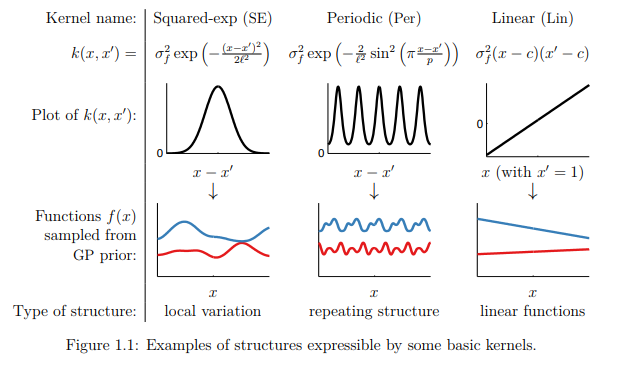
\includegraphics[width=0.7\textwidth]{img/kernels}

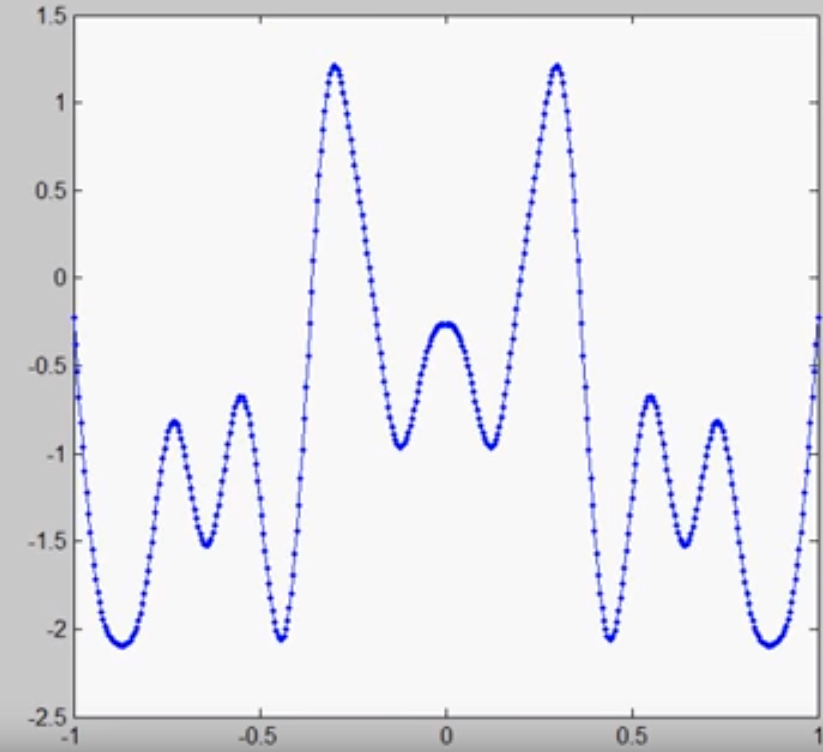
\includegraphics[width=0.7\textwidth]{img/symmetric-kernel}

Image stolen from https://www.cs.toronto.edu/~duvenaud/cookbook/


\begin{tcolorbox}
    \newterm{Gaussian Process} is a \newterm{stochastic process} (a collection of random variables), such that every subset of those random variables has a multivariate Gaussian distribution. It is defined by a mean function $m(x)$ and a covariance funciton $\kappa(x, x')$. Formally, we write \todo{osklive GP}:
    
    \begin{equation}
    f(x) \sim \gN \gG \gP (m(x), \kappa(x, x'))
    \end{equation} \todo{finish}
    
    Bayesian inference ...
    
    \begin{equation}
        \text{posterior} = \frac{\text{likelihood} \times \text{prior}}{\text{evidence}}
    \end{equation},
    
    where evidence is also called \newterm{marginal likelihood}. More concretely, we usually want to compute the posterior distribution over the parameters $\vw$ given the inputs $\mX$ and outputs $\vy$
    
    \begin{equation}
        p(\vw | \vy, \mX) = \frac{p(\vy | \vw, \mX) p(\vw)}{p(\vy | \mX)}
    \end{equation}.
    
    The marginal likelihood is independent of the weights and acts as a normalizing constant. We compute it using marginalization
    
    \begin{equation}
        p(\vy | \mX) = \int p(\vy | \vw, \mX) p(\vw) d \vw.
    \end{equation}
    
    \todo{describe prior over functions}
\end{tcolorbox}


\section{GP from scratch again}



\section{Noise-less Gaussian Process Regression}

\section{Noisy Gaussian Process Regression}


\chapter{TODO Bucket}


\begin{thm}[\citep{murphy2012machine}] (Inverse of a partitioned matrix). Consider a partitioned matrix

\begin{equation}
\mM = \begin{bmatrix} \mA & \mB \\ \mC & \mD \end{bmatrix}
\end{equation}

where we assume $\mA$ and $\mD$ are invertible \todo{staci to? nemusi byt i ty ostatni?}. We have

\begin{equation}
\mM^{-1} = \begin{bmatrix} \mI & \mZero \\ \mI & \mI \end{bmatrix}
\end{equation}
\end{thm}

\begin{proof}
All we need to do is perform a block \newterm{LDU decomposition} and we directly arrive at our solution. We begin by zeroing out $\mB$.

\begin{equation} \label{eq:block-ld-part}
\begin{bmatrix} \mI & -\mB \mD^{-1} & \\ \mZero & \mI \end{bmatrix}
\begin{bmatrix}\mA & \mB \\ \mC & \mD \end{bmatrix} =
\begin{bmatrix} \mA - \mB \mD^{-1} \mC & \mZero \\ \mC & \mD \end{bmatrix}
\end{equation}

The quantity in the top left block is called a \newterm{Schur complement} of $\mM$ wrt $\mD$. We denote it as follows, and also define a variant for the bottom right block

\begin{align}
\mM/\mD &= \mA - \mB \mD^{-1} \mC \\
\mM/\mA &= \mD - \mC \mA^{-1} \mB
\end{align}

Substituting back into \eqref{eq:block-ld-part} we get the following

\begin{equation}
\begin{bmatrix} \mM/\mD & \mZero \\ \mC & \mD \end{bmatrix}
\end{equation}

We follow by eliminating the bottom left block in \eqref{eq:block-ld-part}

\begin{equation} \label{eq:block-du-part}
\begin{bmatrix} \mM/\mD & \mZero \\ \mC & \mD \end{bmatrix}
\begin{bmatrix} \mI & \mZero \\ -\mD^{-1} \mC & \mI \end{bmatrix} =
\begin{bmatrix} \mM/\mD & \mZero \\ \mZero & \mD \end{bmatrix}
\end{equation}

Putting together \eqref{eq:block-ld-part} and \eqref{eq:block-du-part} we get

\begin{equation}
\underbrace{\begin{bmatrix} \mI & -\mB \mD^{-1} & \\ \mZero & \mI \end{bmatrix}}_{\mX}
\underbrace{\begin{bmatrix}\mA & \mB \\ \mC & \mD \end{bmatrix}}_{\mM}
\underbrace{\begin{bmatrix} \mI & \mZero \\ -\mD^{-1} \mC & \mI \end{bmatrix}}_{\mZ} = 
\underbrace{\begin{bmatrix} \mM/\mD & \mZero \\ \mZero & \mD \end{bmatrix}}_{\mW}
\end{equation}

Basic matrix algebra allows us to re-arrange the terms \todo{cite stolen from murphy?}, taking the inverse of both sides

\begin{align}
(\mX \mM \mZ)^{-1} &= \mW^{-1} \\
\mZ^{-1} \mM^{-1} \mX^{-1} &= \mW^{-1} \\
\mM^{-1} &= \mZ \mW^{-1} \mX
\end{align}

Which gives us the final form, making use of the fact that to invert a diagonal matrix we just need to invert its diagonal

\begin{equation} \label{eq:block-inverse}
\mM^{-1} = \begin{bmatrix} \mA & \mB \\ \mC & \mD \end{bmatrix}^{-1} =
\begin{bmatrix} \mI & \mZero \\ -\mD^{-1} \mC & \mI \end{bmatrix}
\begin{bmatrix} (\mM/\mD)^{-1} & \mZero \\ \mZero & \mD^{-1} \end{bmatrix}
\begin{bmatrix} \mI & -\mB \mD^{-1} & \\ \mZero & \mI \end{bmatrix}
\end{equation}

\end{proof}



\section{TODO Linear Gaussian transform - change of variables}

\begin{align}
P(\vx \in \mM) = \int_\mM \frac{1}{(2 \pi)^{D/2} |\mSigma|^{1/2}|} exp \left(-\frac{1}{2} (\vx - \vmu)^T \mSigma^{-1} (\vx - \vmu) \right) d \vx \\
P(\vx \in \mA^{-1} \mM) = \int_{\mA^{-1} \mM} \frac{1}{(2 \pi)^{D/2} |\mSigma|^{1/2}} \exp \left(-\frac{1}{2} (\vu - \vmu)^T \mSigma^{-1} (\vu - \vmu) \right) d \vu \\
\vu = \mA \vx
\end{align}


\chapter{Bayesian Optimization}

Black box optimization of $f(x)$ where the evaluation is costly. Using GP as a
surrogate model. We use an \newterm{acquisition function} to find where the
next sample should be taken.

\section{Acquisition functions}

In each step, the objective function $f$ is sampled at $x_t = \argmax_x
u(x|D_{1:t-1})$ where $u$ is the acquisition function and $D_{1:t-1} =
((x_1,y_1),\ldots,(x_{t-1},y_{t-1}))$.

\begin{defn}
  \newterm{Expected improvement} $EI(x)$ is defined as

  \begin{equation}
    EI(x) = E_{Y \sim \gN(\mu, \sigma^2)} [max(f(x) - f(x^+), 0)]
  \end{equation}

  where $f(x^+)$ is the value of the best sample so far and $x^+ =
  \argmax_{x_i \in x_{1:t}} f(x_i)$.
\end{defn}

\section{Algorithm}

Iteratively for $t = 1,2,\ldots:$ {TODO NANDO}

\begin{itemize}
  \item Solve $x_t = \argmax_x u(x|D_{1:t-1})$ by combining the attributes of
    the posterior distribution in a utility function $u$.
  \item Sample the objective function $y_t = f(x_t) + \epsilon_t$.
  \item Augment the data $D_{1:t} = \set{D_{1:t-1}, (x_t, y_t)}$ and update
    the GP surrogate model based on the new data.
\end{itemize}


\subsection{Probability of Improvement}

We add a small term $\xi$ because otherwise $PI(x^+) = \frac{1}{2}.$

\begin{align}
  PI(x) &= P(f(x) \geq \mu^+ + \xi) \\
        &= \Phi \left(\frac{\mu(x) - \mu^+ - \xi}{\sigma(x)} \right)
\end{align}

where $\Phi$ is the CDF of a Gaussian. If we knew up front what is the best
value $f(x^*)$ we can model that directly by $P(f(x) \geq f(x^*))$.


\subsection{Expected utility}

At iteration $n+1$, choose the point that minimizes the distance to the
objective evaluated at the maximum $x^*$.

\begin{align}
  x_{n+1} &= \argmin_x E(\norm{ \underbrace{f_{n+1}(x)}_{\text{GP}} - \underbrace{f(x^*)}_{\text{true}\ f} } | D_n) \\
          &=\argmin_x \int \norm{f_{n+1}(x) - f(x^*)} p(f_{n+1} | D_n) \diff f_{n+1}
\end{align}

We however don't know the true objective at the maximum. Instead we use (Mockus
et al., 1978 ??? TODO ref) where $f^{\max} = \mu^+ + \xi$

\begin{equation}
  x = \argmax_x E(\max\set{0, f_{n+1}(x) - f^{max}}|D_n)
\end{equation}

which can be solved analytically with

\begin{align}
  EI(x) &= \begin{cases}
    (\mu(x) - \mu^+ - \xi) \Phi(Z) + \sigma(x)\varphi(Z) & if \sigma(x) > 0 \\
    0 & if \sigma(x) = 0
  \end{cases} \\
  Z &= \frac{\mu(x) - \mu^+ - \xi}{\sigma(x)}
\end{align}

where $\phi(\cdot)$ and $\Phi(\cdot)$ denote the PDF and CDF of a normalized Gaussian.


\subsection{GP-UCB}

Define the \newterm{regret} and \newterm{cumulative regret} as follows:

\begin{align}
  r(x) &= f(x^*) - f(x) \\
  R_T &= r(x_1) + \cdots + r(x_T).
\end{align}

The GP-UCB criterion is as follows:

\begin{align}
  GP-UCB(x) = \mu(x) + \sqrt{\nu \beta} \sigma(x)
\end{align}

with $\nu = 1$ and $\beta_t = 2 \log(t^{d/2 + 2}\pi^2 / 3 \delta)$ where it can
be shown with high probability that this method has no regret, i.e. $\lim_{T
\rightarrow \infty} R_T / T = 0$. (Srinivas et at, 2010 TODO REF). (NOTE, if
the set of points is not infinite, $\beta$ ends up being different).


\subsection{Thompson sampling}

Draw a random sample (function) from the posterior, optimize to find its max,
evaluate the true $f(x)$ at the found max.

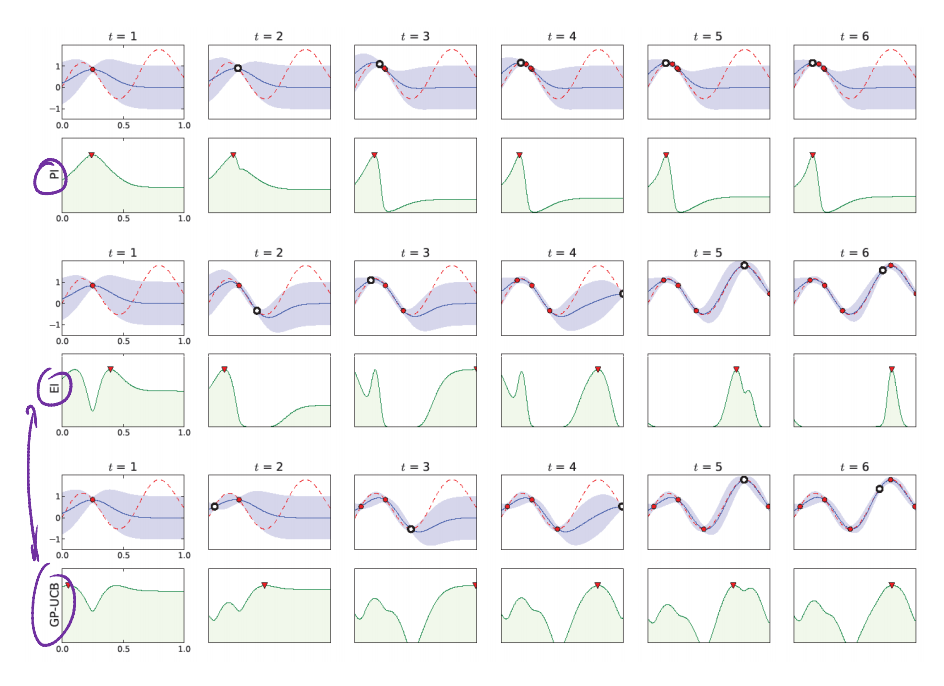
\includegraphics[width=0.9\textwidth]{img/acquisition-functions.png}

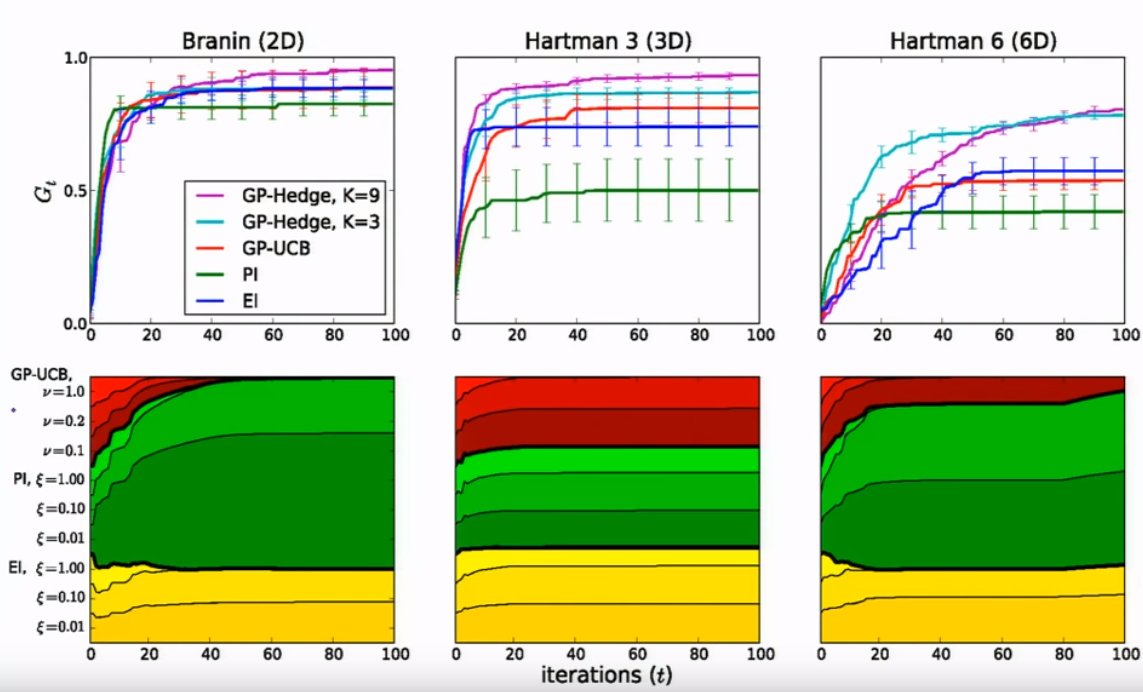
\includegraphics[width=0.9\textwidth]{img/portfolios-of-acquisition-functions.png}


\subsection{Max LCB}

There is no point in sampling where UCB is lower than $\max LCB$ (with high probability).

\chapter{Appendix?}

\section{Cholesky Decomposition}

\begin{defn}
  The \newterm{Cholesky decomposition} is a decomposition of a
  positive definite matrix into a product of a lower triangular matrix and
  its conjugate transpose. Since we will only work with symmetric
  positive-definite matrices we omit the conjugacy and define Cholesky
  decomposition as

  \begin{equation}
    \mA = \mL \mL^T
  \end{equation}

  where $\mL$ is a lower triangular matrix called the \newterm{Cholesky factor}.
\end{defn}

Because of its numerical stability, Cholesky decomposition is useful for
solving systems of linear equations $\mA \vx = \vb$ where $\mA$ is symmetric
and positive definite. We do this by first solving the triangular system $\mL
\vy = \vb$ by forward substitution, and then the triangular system $\mL^T \vx =
\vy$ by back substitution. This works because

\begin{align}
  \mA \vx &= \vb \qquad \text{assuming $\mA$ is symmetric positive-definite} \\
  \mL\mL^T \vx &= \vb \\
  \mL \vy &= \vb \\
  \mL^T \vx &= \vy \qquad \text{which if we back-substitute $\vy$} \\
  \mL (\mL^T \vx) &= \vy \qquad \text{using associativity} \\
  (\mL \mL^T) \vx &= \mA \vx = \vy.
\end{align}

For brevity, we'll apply the MATLAB {TODO ref} backslash operator where $\mA
\backslash \vb = \vx$, which allows us to write the above as $\vx = \mL^T
\backslash (\mL \backslash b)$.


\section{TODO Bucket}

\begin{thm}[\citep{murphy2012machine}] (Inverse of a partitioned matrix).
  Consider a partitioned matrix

  \begin{equation}
    \mM = \begin{bmatrix} \mA & \mB \\ \mC & \mD \end{bmatrix}
  \end{equation}

  where we assume $\mA$ and $\mD$ are invertible {TODO staci to? nemusi byt i
  ty ostatni?}. We have

  \begin{equation}
    \mM^{-1} = \begin{bmatrix} \mI & \mZero \\ \mI & \mI \end{bmatrix}
  \end{equation}
\end{thm}

\begin{proof}
  All we need to do is perform a block \newterm{LDU decomposition} and we
  directly arrive at our solution. We begin by zeroing out $\mB$.

  \begin{equation} \label{eq:block-ld-part}
    \begin{bmatrix} \mI & -\mB \mD^{-1} & \\ \mZero & \mI \end{bmatrix}
    \begin{bmatrix}\mA & \mB \\ \mC & \mD \end{bmatrix} =
    \begin{bmatrix} \mA - \mB \mD^{-1} \mC & \mZero \\ \mC & \mD \end{bmatrix}
  \end{equation}

  The quantity in the top left block is called a \newterm{Schur complement} of
  $\mM$ wrt $\mD$. We denote it as follows, and also define a variant for the
  bottom right block

  \begin{align}
    \mM/\mD &= \mA - \mB \mD^{-1} \mC \\
    \mM/\mA &= \mD - \mC \mA^{-1} \mB
  \end{align}

  Substituting back into \eqref{eq:block-ld-part} we get the following

  \begin{equation}
    \begin{bmatrix} \mM/\mD & \mZero \\ \mC & \mD \end{bmatrix}
  \end{equation}

  We follow by eliminating the bottom left block in \eqref{eq:block-ld-part}

  \begin{equation} \label{eq:block-du-part}
    \begin{bmatrix} \mM/\mD & \mZero \\ \mC & \mD \end{bmatrix}
    \begin{bmatrix} \mI & \mZero \\ -\mD^{-1} \mC & \mI \end{bmatrix} =
    \begin{bmatrix} \mM/\mD & \mZero \\ \mZero & \mD \end{bmatrix}
  \end{equation}

  Putting together \eqref{eq:block-ld-part} and \eqref{eq:block-du-part} we get

  \begin{equation}
    \underbrace{\begin{bmatrix} \mI & -\mB \mD^{-1} & \\ \mZero & \mI \end{bmatrix}}_{\mX}
    \underbrace{\begin{bmatrix}\mA & \mB \\ \mC & \mD \end{bmatrix}}_{\mM}
    \underbrace{\begin{bmatrix} \mI & \mZero \\ -\mD^{-1} \mC & \mI \end{bmatrix}}_{\mZ} =
    \underbrace{\begin{bmatrix} \mM/\mD & \mZero \\ \mZero & \mD \end{bmatrix}}_{\mW}
  \end{equation}

  Basic matrix algebra allows us to re-arrange the terms {TODO cite stolen from
  murphy?}, taking the inverse of both sides

  \begin{align}
    (\mX \mM \mZ)^{-1} &= \mW^{-1} \\
    \mZ^{-1} \mM^{-1} \mX^{-1} &= \mW^{-1} \\
    \mM^{-1} &= \mZ \mW^{-1} \mX
  \end{align}

  Which gives us the final form, making use of the fact that to invert a
  diagonal matrix we just need to invert its diagonal

  \begin{equation} \label{eq:block-inverse}
    \mM^{-1} = \begin{bmatrix} \mA & \mB \\ \mC & \mD \end{bmatrix}^{-1} =
    \begin{bmatrix} \mI & \mZero \\ -\mD^{-1} \mC & \mI \end{bmatrix}
    \begin{bmatrix} (\mM/\mD)^{-1} & \mZero \\ \mZero & \mD^{-1} \end{bmatrix}
    \begin{bmatrix} \mI & -\mB \mD^{-1} & \\ \mZero & \mI \end{bmatrix}
  \end{equation}

\end{proof}



\section{TODO Linear Gaussian transform}

\todo{change of variables}

\begin{align}
  P(\vx \in \mM) = \int_\mM \frac{1}{(2 \pi)^{D/2} |\mSigma|^{1/2}|} exp \left(-\frac{1}{2} (\vx - \vmu)^T \mSigma^{-1} (\vx - \vmu) \right) d \vx \\
  P(\vx \in \mA^{-1} \mM) = \int_{\mA^{-1} \mM} \frac{1}{(2 \pi)^{D/2} |\mSigma|^{1/2}} \exp \left(-\frac{1}{2} (\vu - \vmu)^T \mSigma^{-1} (\vu - \vmu) \right) d \vu \\
  \vu = \mA \vx
\end{align}

% TODO TODO tohle mozna patri nekam jako summary.
% the parameters are {TODO zkontrolovat kde je $\mu$ a chybi tam vector}
%
% \begin{align}
%   \vmu_{1|2} &= \vmu_1 - \ms{12} \ms{22}^{-1} (\vx_2 - \vmu_2) \\
%   \ms{1|2} &= \mSigma / \ms{22} = \ms{11} - \ms{12} \ms{22}^{-1} \ms{21}
% \end{align}


% TODO: inversion lemma proof vykopirovany jako zaloha
% \begin{proof}
%   All we need to do is perform a block \newterm{LDU decomposition} and we
%   directly arrive at our solution. We begin by zeroing out $\mB$.
%
%   \begin{equation} \label{eq:block-ld-part}
%     \begin{bmatrix} \mI & -\mB \mD^{-1} & \\ \mZero & \mI \end{bmatrix}
%     \begin{bmatrix}\mA & \mB \\ \mC & \mD \end{bmatrix} =
%     \begin{bmatrix} \mA - \mB \mD^{-1} \mC & \mZero \\ \mC & \mD \end{bmatrix}
%   \end{equation}
%
%   The quantity in the top left block is called a \newterm{Schur complement} of
%   $\mM$ wrt $\mD$. We denote it as follows, and also define a variant for the
%   bottom right block
%
%   \begin{align}
%     \mM/\mD &= \mA - \mB \mD^{-1} \mC \\
%     \mM/\mA &= \mD - \mC \mA^{-1} \mB
%   \end{align}
%
%   Substituting back into \eqref{eq:block-ld-part} we get the following
%
%   \begin{equation}
%     \begin{bmatrix} \mM/\mD & \mZero \\ \mC & \mD \end{bmatrix}
%   \end{equation}
%
%   We follow by eliminating the bottom left block in \eqref{eq:block-ld-part}
%
%   \begin{equation} \label{eq:block-du-part}
%     \begin{bmatrix} \mM/\mD & \mZero \\ \mC & \mD \end{bmatrix}
%     \begin{bmatrix} \mI & \mZero \\ -\mD^{-1} \mC & \mI \end{bmatrix} =
%     \begin{bmatrix} \mM/\mD & \mZero \\ \mZero & \mD \end{bmatrix}
%   \end{equation}
%
%   Putting together \eqref{eq:block-ld-part} and \eqref{eq:block-du-part} we get
%
%   \begin{equation}
%     \underbrace{\begin{bmatrix} \mI & -\mB \mD^{-1} & \\ \mZero & \mI \end{bmatrix}}_{\mX}
%     \underbrace{\begin{bmatrix}\mA & \mB \\ \mC & \mD \end{bmatrix}}_{\mM}
%     \underbrace{\begin{bmatrix} \mI & \mZero \\ -\mD^{-1} \mC & \mI \end{bmatrix}}_{\mZ} =
%     \underbrace{\begin{bmatrix} \mM/\mD & \mZero \\ \mZero & \mD \end{bmatrix}}_{\mW}
%   \end{equation}
%
%   Basic matrix algebra allows us to re-arrange the terms {TODO cite stolen from
%   murphy?}, taking the inverse of both sides
%
%   \begin{align}
%     (\mX \mM \mZ)^{-1} &= \mW^{-1} \\
%     \mZ^{-1} \mM^{-1} \mX^{-1} &= \mW^{-1} \\
%     \mM^{-1} &= \mZ \mW^{-1} \mX
%   \end{align}
%
%   Which gives us the final form, making use of the fact that to invert a
%   diagonal matrix we just need to invert its diagonal
%
%   \begin{equation} \label{eq:block-inverse}
%     \mM^{-1} = \begin{bmatrix} \mA & \mB \\ \mC & \mD \end{bmatrix}^{-1} =
%     \begin{bmatrix} \mI & \mZero \\ -\mD^{-1} \mC & \mI \end{bmatrix}
%     \begin{bmatrix} (\mM/\mD)^{-1} & \mZero \\ \mZero & \mD^{-1} \end{bmatrix}
%     \begin{bmatrix} \mI & -\mB \mD^{-1} & \\ \mZero & \mI \end{bmatrix}
%   \end{equation}
%
% \end{proof}


\chapter*{Conclusion}
\addcontentsline{toc}{chapter}{Conclusion}


%%% Bibliography
%%% Bibliography (literature used as a source)
%%%
%%% We employ bibTeX to construct the bibliography. It processes
%%% citations in the text (e.g., the \cite{...} macro) and looks up
%%% relevant entries in the bibliography.bib file.
%%%
%%% The \bibliographystyle command selects, which style will be used
%%% for references from the text. The argument in curly brackets is
%%% the name of the corresponding style file (*.bst). Both styles
%%% mentioned in this template are included in LaTeX distributions.

\bibliographystyle{plainnat}    %% Author (year)
% \bibliographystyle{unsrt}     %% [number]

\renewcommand{\bibname}{Bibliography}

%%% Generate the bibliography. Beware that if you cited no works,
%%% the empty list will be omitted completely.

\bibliography{bibliography}

%%% If case you prefer to write the bibliography manually (without bibTeX),
%%% you can use the following. Please follow the ISO 690 standard and
%%% citation conventions of your field of research.

% \begin{thebibliography}{99}
%
% \bibitem{lamport94}
%   {\sc Lamport,} Leslie.
%   \emph{\LaTeX: A Document Preparation System}.
%   2nd edition.
%   Massachusetts: Addison Wesley, 1994.
%   ISBN 0-201-52983-1.
%
% \end{thebibliography}


%%% Figures used in the thesis (consider if this is needed)
\listoffigures

%%% Tables used in the thesis (consider if this is needed)
%%% In mathematical theses, it could be better to move the list of tables to the beginning of the thesis.
\listoftables

%%% Abbreviations used in the thesis, if any, including their explanation
%%% In mathematical theses, it could be better to move the list of abbreviations to the beginning of the thesis.
\chapwithtoc{List of Abbreviations}

%%% Attachments to the master thesis, if any. Each attachment must be
%%% referred to at least once from the text of the thesis. Attachments
%%% are numbered.
%%%
%%% The printed version should preferably contain attachments, which can be
%%% read (additional tables and charts, supplementary text, examples of
%%% program output, etc.). The electronic version is more suited for attachments
%%% which will likely be used in an electronic form rather than read (program
%%% source code, data files, interactive charts, etc.). Electronic attachments
%%% should be uploaded to SIS and optionally also included in the thesis on a~CD/DVD.
%%% Allowed file formats are specified in provision of the rector no. 72/2017.
\appendix
\chapter{Attachments}

\section{First Attachment}

\printindex

\openright
\end{document}
